\documentclass[lang=cn,10pt]{elegantbook}

\title{Dx的复变函数 }


\author{DX}

\date{2025.8.19}


\extrainfo{不要以为抹消过去，重新来过，即可发生什么改变。—— 比企谷八幡}

\setcounter{tocdepth}{3}

\logo{logo-blue.png}
\cover{cover.jpg}

% 本文档命令

\usepackage{tikz-3dplot}
\usepackage{tikz}
\usepackage{array}
\newcommand{\ccr}[1]{\makecell{{\color{#1}\rule{1cm}{1cm}}}}

% 修改标题页的橙色带
% \definecolor{customcolor}{RGB}{32,178,170}
% \colorlet{coverlinecolor}{customcolor}

\begin{document}

\maketitle
\frontmatter

\tableofcontents

\mainmatter
\chapter{复变函数基础知识}
\begin{dxtips}{学复变函数的目的——升维简化问题}[PS]\label{dx:any-construct}
今天是8.23，我突然想到复数，复变函数相等于升维，我们知道求导其实就是一种降维，信息会减少，复杂度上升。那么升维，会有更多的信息, 可以让问题比较简单。- 降维 → 找到核心规律或约束，让问题变得更可控、更优雅。
    - 升维 → 提供更丰富的视角或结构，问题看得更全面。
\end{dxtips}
\section{收敛性}
\begin{theorem}
    

根据上面所提到的复数的算术和几何性质，得到复数的收敛和极限的重要概念。

序列 $\{z_1, z_2, \cdots\}$，若存在 $w \in \mathbb{C}$ 使得
\[
\lim_{n \to +\infty} |z_n - w| = 0 
\quad (\text{或者 } w = \lim_{n\to+\infty} z_n),
\]
则称序列 $\{z_1, z_2, \cdots\}$ 收敛于 $w$。

以上收敛的概念并不是新的定义。事实上，因为复数集 $\mathbb{C}$ 中的绝对值和欧几里得平面 $\mathbb{R}^2$ 中定义的距离是一致的，所以序列 $\{z_n\}$ 收敛于 $w$ 当且仅当序列在复平面上对应的点列收敛于 $w$ 在复平面中对应的点。

特别地，序列 $\{z_n\}$ 收敛于 $w$ 当且仅当 $\{z_n\}$ 的实部序列和虚部序列分别收敛于 $w$ 的实部和虚部。\\
复数的收敛性和实数不同的是，实数都在数轴上收敛只有两个方向，但是复数收敛是得平面各个方向都保证收敛。
\end{theorem}
\begin{theorem}
    若得不到序列确切的收敛值（例如 $\lim\limits_{N\to+\infty} \sum\limits_{n=1}^N \tfrac{1}{n^3}$），
此时也可以由序列本身来描述收敛。序列 $\{z_n\}$ 称为柯西列（或基本列），
当 $n,m \to +\infty$ 时，
\[
|z_n - z_m| \to 0.
\]

也就是说，任给 $\varepsilon > 0$，总存在 $N > 0$，当 $n,m > N$ 时，总有 $|z_n - z_m| < \varepsilon$。
实分析中一个很重要的结论是：实数集 $\mathbb{R}$ 是完备的，实数集中的任何柯西列都收敛。
\end{theorem}
\section{复平面是完备的}
\begin{proposition}
    

  在复平面中，若 $z_0 \in \mathbb{C}, r>0$，则称
\[
D_r(z_0) = \{ z \in \mathbb{C} : |z-z_0| < r \}
\]
为以 $z_0$ 为中心、$r$ 为半径的开圆盘；相应的闭圆盘定义为
\[
\overline{D}_r(z_0) = \{ z \in \mathbb{C} : |z-z_0| \leq r \},
\]
其边界圆周记为
\[
C_r(z_0) = \{ z \in \mathbb{C} : |z-z_0| = r \}.
\]
特别地，以原点为中心、半径为 $1$ 的开圆盘称为单位圆盘，记作
\[
D = \{ z \in \mathbb{C} : |z| < 1 \}.
\]
若集合 $\Omega \subset \mathbb{C}$，存在 $r>0$ 使得 $D_r(z_0) \subset \Omega$，则称 $z_0$ 为 $\Omega$ 的内点，所有内点组成的集合称为 $\Omega$ 的内部。若 $\Omega$ 的所有点都是内点，则称 $\Omega$ 为开集。  
\end{proposition}
\begin{proposition}
    如果集合 $\Omega$ 的余集 $\Omega^c = \mathbb{C} - \Omega$ 是开集，那么集合 $\Omega$ 称为闭集。  
这个性质可以按照极限点更好地描述：如果存在序列 $z_n \in \Omega$，且总有 $z_n \neq z$，使得 
\[
\lim_{n\to +\infty} z_n = z,
\]
则称点 $z \in \mathbb{C}$ 是集合 $\Omega$ 中的极限点。  
读者容易证明集合为闭集当且仅当该集合包含了它所有的极限点。  

集合 $\Omega$ 的闭包是由集合 $\Omega$ 与它的极限点合并构成的，通常记为 $\overline{\Omega}$。  
集合 $\Omega$ 的边界等于它的闭包减去它的内部，通常记为 $\partial \Omega$。  

集合 $\Omega$ 有界等价于存在 $M>0$ 使得任意的 $z \in \Omega$ 均满足 $|z| < M$。  
也就是说，集合 $\Omega$ 必包含在某个大的圆周内。  
如果集合 $\Omega$ 有界，定义它的直径为
\[
\mathrm{diam}(\Omega) = \sup_{z,w \in \Omega} |z-w|.
\]

有界闭集 $\Omega$ 称为紧的。
\end{proposition}
\begin{theorem}[1.2]
集合 $\Omega \subset \mathbb{C}$ 是紧的充要条件是任意柯西列 
$\{z_n\} \subset \Omega$ 均有收敛于 $\Omega$ 的子列。
\end{theorem}

集合 $\Omega$ 的开覆盖是指存在开集族 $\{U_\alpha\}$ （不一定可数），
使得
\[
\Omega \subset \bigcup_{\alpha} U_\alpha.
\]
\begin{theorem}[1.3]
集合 $\Omega$ 是紧的充要条件是 $\Omega$ 的任意开覆盖中必可选出一个有限子覆盖。
\end{theorem}
\begin{theorem}[1.4]
如果 $\Omega_1 \supset \Omega_2 \supset \cdots \supset \Omega_n \supset \cdots$ 
是复数集 $\mathbb{C}$ 中的非空紧集序列，当 $n \to +\infty$ 时，
\[
\mathrm{diam}(\Omega_n) \to 0,
\]
那么一定存在唯一的 $w \in \mathbb{C}$，使得对所有的 $n$，有 $w \in \Omega_n$。
\end{theorem}

\begin{proof}
在每个 $\Omega_n$ 中选择一个 $z_n$。根据条件 $\mathrm{diam}(\Omega_n) \to 0$，
则 $\{z_n\}$ 是柯西列，因此 $\{z_n\}$ 一定收敛于某个极限值，不妨设该极限为 $w$。
又因为 $\Omega_n$ 为紧集，所以对所有的 $n$，有 $w \in \Omega_n$。

下面证明 $w$ 的唯一性。假设存在 $w'$ 也满足条件，且 $w' \neq w$，
那么 $|w-w'| > 0$。这与 $\mathrm{diam}(\Omega_n) \to 0$ 矛盾，即 $w$ 是唯一的。
\end{proof}
关于紧还有一个很重要的性质，就是嵌套集。这个结论不但在第 2 章的 Gour-sat 定理的证明中用到，早在开始研究复值函数数论时就已经用过。
这个定理可以验证实数轴是紧集——有限覆盖定理。海涅–博雷尔定理把它具体化了：在实数轴里，紧集 就是 闭 + 有界。
\begin{proposition}[连通的意义]
    最后要介绍的概念是连通性。开集 $\Omega \subset \mathbb{C}$ 是\textbf{连通的}，
即如果它不能分成两个不相交的非空开集 $\Omega_1, \Omega_2$，使得
\[
\Omega = \Omega_1 \cup \Omega_2.
\]

复数集 $\mathbb{C}$ 中连通的开集称为\textbf{区域}。
类似地，闭集 $F$ 是\textbf{连通的}，即如果它不能分成两个不相交的非空闭集
$F_1, F_2$，使得 $F = F_1 \cup F_2$。

连通性还可以等价地用曲线描述，这种描述应用更广泛：
$\Omega$ 是连通的开集，当且仅当 $\Omega$ 中的任意两点都可以由
包含于 $\Omega$ 内的某条曲线 $\gamma$ 连接起来。
\end{proposition}
\section{复数运算的意义}
\begin{figure}[htbp]
    \centering
    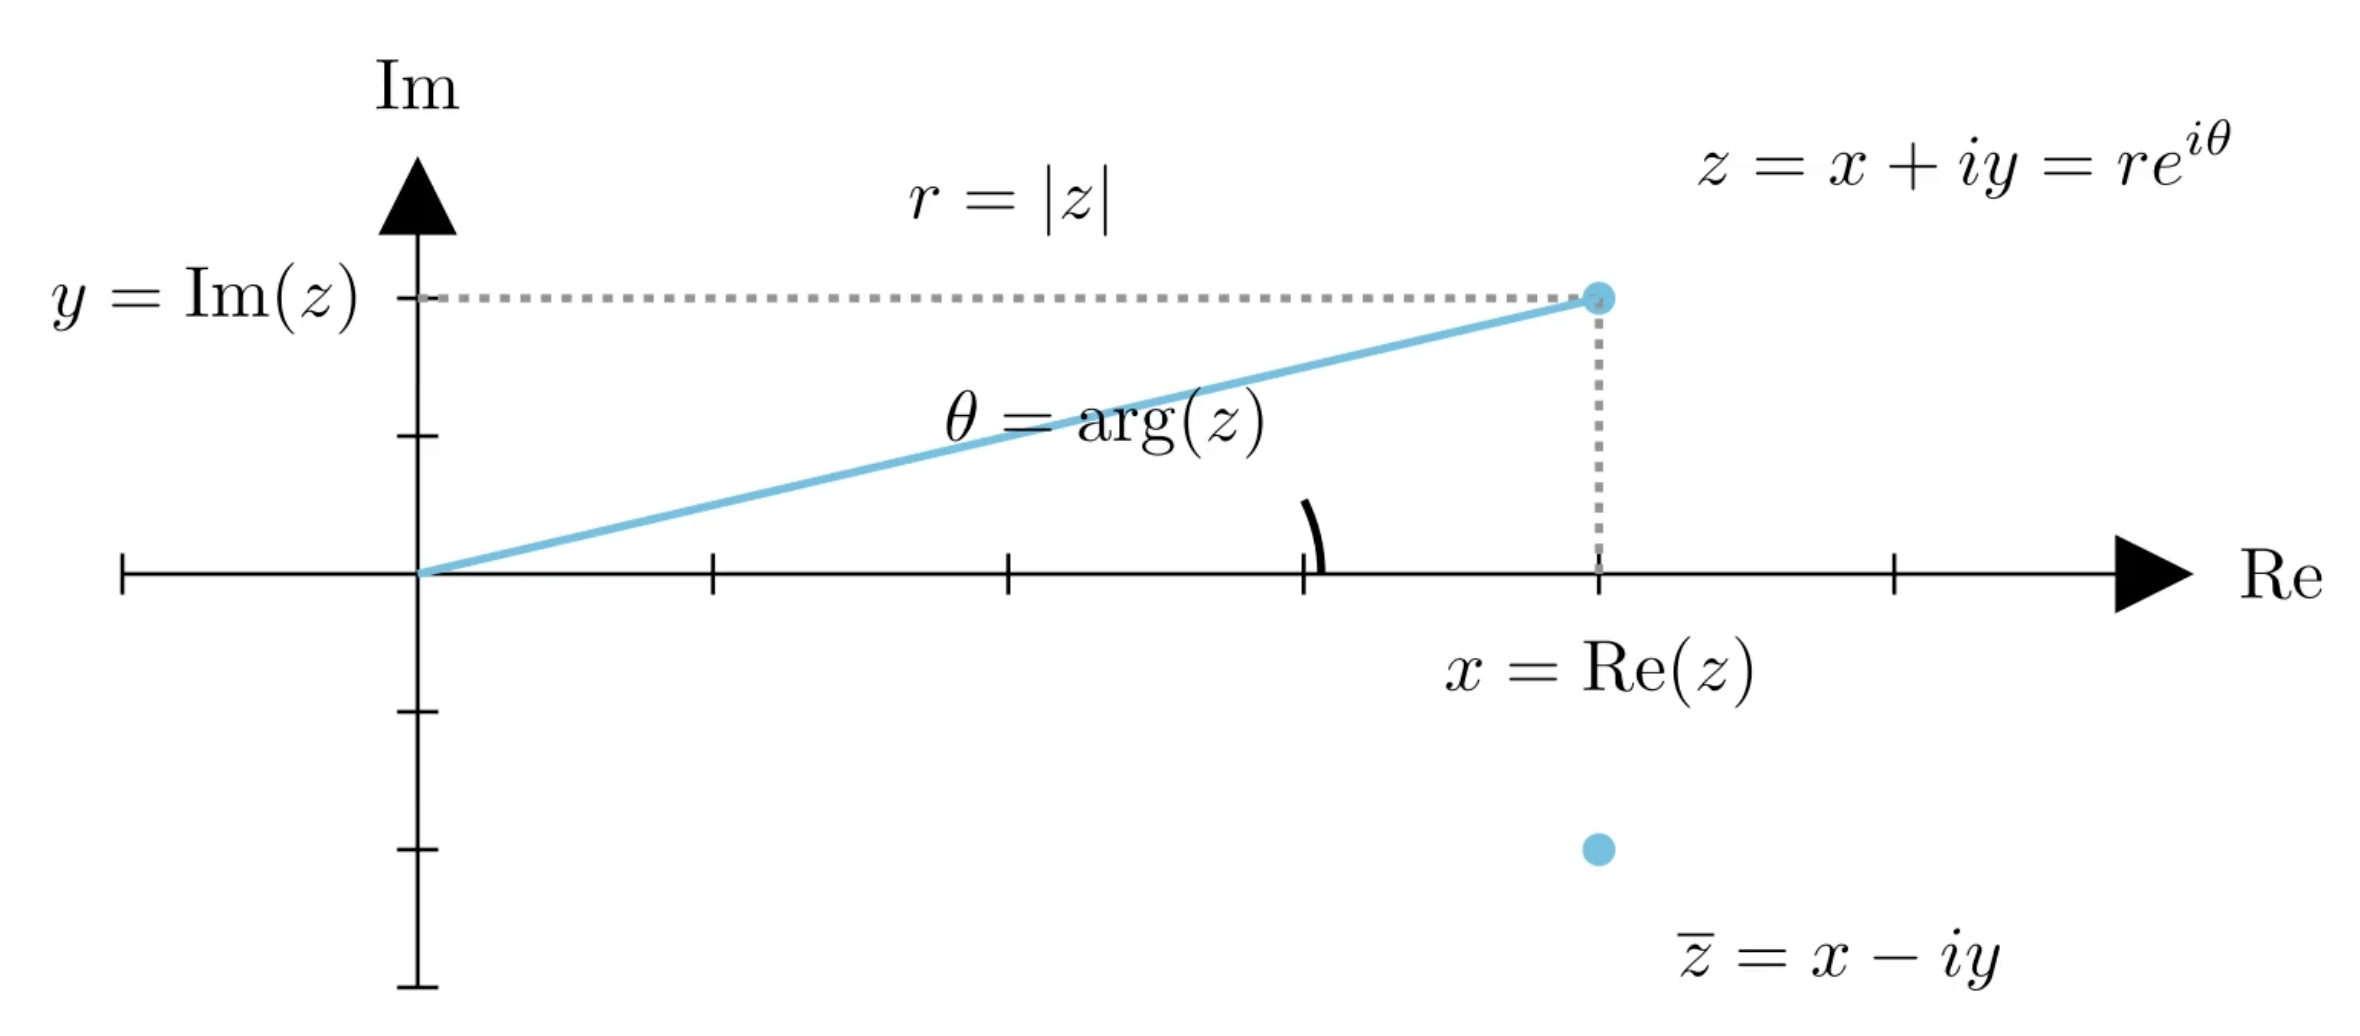
\includegraphics[width=0.7\linewidth]{image.png}
    \caption{示意图：复数的几何表示}
    \label{fig:complex-plane}
\end{figure}
arg(z)是主辐射角。
\begin{theorem}[复数的意义]
 
\[
\operatorname{Re}(z)=\tfrac12\,(z+\overline{z}) \qquad
\operatorname{Im}(z)=\tfrac{1}{2i}\,(z-\overline{z}) \qquad
|z|=\sqrt{x^2+y^2}
\]

\[
\tan(\arg z)=\frac{\operatorname{Im}(z)}{\operatorname{Re}(z)} \qquad
re^{i\theta}=r(\cos\theta+i\sin\theta)
\]

\[
\overline{\overline{z}}=z \qquad
|z_1z_2|=|z_1|\,|z_2| \qquad
\left|\frac{z_1}{z_2}\right|=\frac{|z_1|}{|z_2|}\ (z_2\neq0)
\]

\[
\overline{z_1\pm z_2}=\overline{z_1}\pm\overline{z_2} \qquad
\overline{z_1z_2}=\overline{z_1}\,\overline{z_2} \qquad
\overline{\!\left(\frac{z_1}{z_2}\right)\!}=\frac{\overline{z_1}}{\overline{z_2}}\ (z_2\neq0)
\]

\[
|z_1\pm z_2|\le |z_1|+|z_2| \qquad
\bigl||z_1|-|z_2|\bigr|\le |z_1\pm z_2|
\]

以下称为广义三角不等式：
\[
|z_1+z_2+\cdots+z_n|\le |z_1|+|z_2|+\cdots+|z_n|.
\]


\end{theorem}

\begin{dxtips}
    实部就是 $x$ 坐标，虚部就是 $y$ 坐标，模长就是向量的长度，$\tan\theta = \tfrac{y}{x}$ 表示斜率。  
复数 $z = re^{i\theta}$ 中，$r$ 是模长，$\theta$ 是向量从 $x$ 轴正半轴旋转的角度。  
共轭就是沿着 $x$ 轴对折。  

向量模长的和大于向量和的模长，符合三角形不等式。  
有共轭时一般不可导。  

辐角 $\mathrm{Arg}(z) = \theta + 2k\pi$。  
辐角 $\theta$ 是向量 $\overrightarrow{OP}$ 与 $x$ 轴正半轴的夹角。  

$-\pi$ 到 $\pi$ 之间的值称为辐角的主值。  

通过 $\arctan \tfrac{y}{x}$ 可以求出辐角，再根据象限来判断辐角应大于 $0$ 还是小于 $0$。  

复数不能比较大小。复数相乘就是模相乘+辐角相加——放缩+旋转
\end{dxtips}
\begin{theorem}[复数的运算法则]
    设复数 $z_1 = x_1 + i y_1,\; z_2 = x_2 + i y_2$，则  

(1) 复数的和与差  
\[
z_1 \pm z_2 = (x_1 \pm x_2) + i (y_1 \pm y_2)
\]

(2) 复数的积  
\[
z_1 \cdot z_2 = (x_1 x_2 - y_1 y_2) + i (x_1 y_2 + x_2 y_1)
\]

(3) 复数的商  
\[
\frac{z_1}{z_2} = 
\frac{x_1 x_2 + y_1 y_2}{x_2^2 + y_2^2}
+ i \, \frac{x_2 y_1 - x_1 y_2}{x_2^2 + y_2^2}
\]
\end{theorem}
\begin{theorem}[复平面的代数运算的基本运算律。]
    \begin{itemize}
  \item \textbf{交换律}：对任意的 $z_1, z_2 \in \mathbb{C}$，有
  \[
  z_1 + z_2 = z_2 + z_1, \quad z_1 z_2 = z_2 z_1.
  \]

  \item \textbf{结合律}：对任意的 $z_1, z_2, z_3 \in \mathbb{C}$，有
  \[
  (z_1+z_2)+z_3 = z_1+(z_2+z_3), \quad (z_1 z_2)z_3 = z_1(z_2 z_3).
  \]

  \item \textbf{分配律}：对任意的 $z_1, z_2, z_3 \in \mathbb{C}$，有
  \[
  z_1(z_2+z_3) = z_1 z_2 + z_1 z_3.
  \]
\end{itemize}

显然，复数的加法相当于平面 $\mathbb{R}^2$ 中二维向量的加法，而复数的乘法则相当于引入了带有伸缩的旋转。事实上，可以引入极坐标来表示复数，观察到某个复数与 $i$ 相乘，则相当于该复数按逆时针方向旋转 $\pi/2$。

复数的模或绝对值与欧几里得（Euclidean）平面 $\mathbb{R}^2$ 中的模长的定义是一致的。通常，复数 $z = x + iy$ 的绝对值定义为
\[
|z| = (x^2+y^2)^{1/2},
\]
所以 $|z|$ 恰好是点 $(x,y)$ 到原点的距离。

特别地，对任意 $z, w \in \mathbb{C}$，均满足三角不等式：
\[
|z+w| \leq |z| + |w|.
\]
\end{theorem}


复数乘法 $(a+bi)(c+di) = $\textcolor{red}{$(ac - bd) + (ad + bc)i$。 } 看见红色字就要想到矩阵。
可以把它理解成矩阵乘法，然后再退回到复数形式。  

复数的模与辐角表示为  
\[
z = a + bi = r(\cos\theta + i \sin\theta) = r e^{i\theta}.
\]  

例如  
\[
1+i = \sqrt{2}\, e^{i \pi/4}, 
\qquad e^{i\pi} = -1.
\]  

复数相乘时，模相乘，辐角相加：  
\[
z_1 z_2 = r_1 e^{i\theta_1} \cdot r_2 e^{i\theta_2} = (r_1 r_2) e^{i(\theta_1+\theta_2)}.
\]  

为了说明 $(ac-bd,\, ad+bc)$ 的由来，可以用矩阵方式：  
\[
\begin{pmatrix}
a & -b \\
b & a
\end{pmatrix}
\begin{pmatrix}
c \\ d
\end{pmatrix}
=
\begin{pmatrix}
ac - bd \\
ad + bc
\end{pmatrix}.
\]  

进一步设 $a = r \cos\theta, \; b = r \sin\theta$，得到  
\[
\begin{pmatrix}
ac - bd \\
ad + bc
\end{pmatrix}
=
r
\begin{pmatrix}
\cos\theta & -\sin\theta \\
\sin\theta & \cos\theta
\end{pmatrix}
\begin{pmatrix}
c \\ d
\end{pmatrix}.
\]  

这说明复数乘法可以看作旋转加缩放。
旋转矩阵
\[
\begin{pmatrix}
\cos\theta & -\sin\theta \\
\sin\theta & \cos\theta
\end{pmatrix}
\]
表示点绕原点逆时针旋转 $\theta$ 角度。缩放因子 $r$ 则表示坐标整体放大或缩小，$r>1$ 放大，$r<1$ 缩小。

例如点 $(1,0)$，在旋转角度 $\theta = \tfrac{\pi}{2}$ 且 $r=1$ 时，旋转矩阵为
\[
\begin{pmatrix}
0 & -1 \\
1 & 0
\end{pmatrix}.
\]
与 $(1,0)$ 相乘：
\[
\begin{pmatrix}
0 & -1 \\
1 & 0
\end{pmatrix}
\begin{pmatrix}
1 \\ 0
\end{pmatrix}
=
\begin{pmatrix}
0 \\ 1
\end{pmatrix}.
\]
这表明点 $(1,0)$ 经过 $90^\circ$ 旋转变换成了 $(0,1)$。由此可见，矩阵乘法能够实现任意角度的旋转与缩放，这也解释了复数运算中为什么辐角需要相加。
\begin{dxtips}[最重要tip]
    虚部总是和旋转有关，复变函数是向量到向量。所以写成 $re^{i\theta}$ 可以看清模长和旋转。

函数极限和实数域一样，只是 $|z-z_0|<\delta$ 是各个方向趋近 $z_0$ 了，
并且 $|f(z)-\alpha|<\varepsilon$，$\delta$ 和 $\varepsilon$ 有关。

有极限的充要条件：实部和虚部分别趋近于它们该去的极限。
\end{dxtips}
\begin{theorem}[乘幂与开方]
   乘积公式
\[
z^n = |z|^n \bigl[\cos(n \,\mathrm{Arg}z) + i \sin(n \,\mathrm{Arg}z)\bigr]
\]
如果令 $|z|=1$，则有
\[
\bigl(\cos(\mathrm{Arg}z) + i \sin(\mathrm{Arg}z)\bigr)^n 
= \cos(n \,\mathrm{Arg}z) + i \sin(n \,\mathrm{Arg}z),
\]
称为 \textbf{De Moivre 公式}。  

如果定义负整数幂为 $z^{-n} = \dfrac{1}{z^n}$，那么 De Moivre 公式仍然成立（同样可用归纳法证明）：  
\[
\bigl(\cos(\mathrm{Arg}z) + i \sin(\mathrm{Arg}z)\bigr)^n 
= \cos(n \,\mathrm{Arg}z) + i \sin(n \,\mathrm{Arg}z), 
\quad \forall n \in \mathbb{Z}.
\] 
由 De Moivre 公式可得复数的开方公式：  

设 $z = r(\cos \theta + i \sin \theta)$，其中 $r=|z|$, $\theta = \mathrm{Arg}z$，  
则 $z$ 的 $n$ 次方根为
\[
w_k = \sqrt[n]{r}\left[\cos\!\left(\frac{\theta + 2k\pi}{n}\right) 
+ i \sin\!\left(\frac{\theta + 2k\pi}{n}\right)\right], 
\quad k=0,1,\dots,n-1.
\]

因此，$z$ 一共有 $n$ 个不同的 $n$ 次方根，它们在复平面上均匀分布在一个圆周上。
\end{theorem}
\begin{definition}
设 $E$ 是复平面 $\mathbb{C}$ 上的点集。如果有一个确定的法则 $f$，使得  
\[
\forall z = x + iy \in E, \quad \exists w = u + iv \in \mathbb{C}
\]
与之对应，我们就把 $f$ 称为在 $E$ 上确定的复变函数。  

这里 $x, y, u, v \in \mathbb{R}$。
\end{definition}
只是存在没有说不能一对多 比如说辐角方根

多值要分解成单值分支

极限连续指是单值函数

z，w一一对应单值复变函数
\begin{dxtips}
    复数是一个向量映射到另一个向量
\end{dxtips}
\textbf{例4：} 作出复平面 $\mathbb{C}$ 上过不共线三点 $a,b,c$ 的圆的表达式。  

若 $z$ 位于 $a,b$ 之间且与 $c$ 同侧弧上，则有  
\[
\Arg \frac{z-a}{z-b} = \theta + 2k\pi \quad (k \in \mathbb{Z}),
\]
\[
\Arg \frac{c-a}{c-b} = \theta + 2k'\pi \quad (k' \in \mathbb{Z}).
\]

因此可以得到条件  
\[
\Arg \left( \frac{z-a}{z-b} \;\Big/ \;\frac{c-a}{c-b} \right) = 2k\pi \quad (k \in \mathbb{Z}).
\]

这即为复平面上过三点 $a,b,c$ 的圆的复数表达式。
两个夹角可以用商的辐角来确定

维度可以用属性来理解一个点身高体重眼睛大小。

\begin{proposition}[引入复球面为了把无穷原点加入]
    
很多多值函数
在点坐标是 $(x,y,u)$ 的三维空间中，把 $xOy$ 平面看作是复平面
\[
z = x + iy.
\]
考虑球面 $S$：
\[
x^2 + y^2 + u^2 = 1.
\]

取定球面上一点 $N(0,0,1)$，称为球极。作连接 $N$ 与 $xOy$ 平面上一点 $A(x,y,0)$ 的直线，
并且设这直线与球面的交点是 $A'(x',y',u')$。那么称 $A'$ 为 $A$ 在球面上的球极投影。$A'$与OA向量的关系如下
\[
x' = \frac{z + \bar{z}}{|z|^2 + 1}, \quad
y' = \frac{z - \bar{z}}{i\,(|z|^2 + 1)}, \quad
u' = \frac{|z|^2 - 1}{|z|^2 + 1}
\]
\end{proposition}
\begin{proof}
    
由于$A$，$A'$，$N$共线，他们的组成的向量共线有比例关系。
x:y:-1=x':y':u'-1
z是OA向量，\\我们现在要求出$x
',y',u'$
\[
z = x + iy = \frac{x'}{1-u'} + i \frac{y'}{1-u'}.
\]

又因
\[
|z|^2 = z \overline{z} = \frac{(x')^2+(y')^2}{(1-u')^2}
= \frac{1-(u')^2}{(1-u')^2} = \frac{1+u'}{1-u'},
\]
于是有
\[
z = \frac{x'+iy'}{1-u'}, 
\qquad
u' = \frac{|z|^2-1}{|z|^2+1}.
\]
\[
x = \frac{z + \bar{z}}{2}, \qquad
y = \frac{z - \bar{z}}{2i}
\]用比例关系算出x',y'
\end{proof}
点离 $N$ 越近，模长越长；离无穷远就有无穷长的模。  
这样，复平面 $\mathbb{C}$ 与 $S-\{N\}$ 之间建立了一个双射。\[
f(z) = \left( \frac{z + \bar{z}}{|z|^2 + 1},\; 
             \frac{z - \bar{z}}{i(|z|^2 + 1)},\; 
             \frac{|z|^2 - 1}{|z|^2 + 1} \right)
\]
\begin{dxtips}[映射与抽代]
你看我们为了我们的目的，或为了更直观，或为了简化问题会构造映射。抽象代数就是为了探究我们构造的映射的结构好不好，同构就是保证我在原像集中a和b操作产生的c映射过去和像集a'和b‘进行对应的运算产生的是不是一个东西。如果是同一个东西我们可能在像像集很难算出a’和b'的结果那么我们就可以原像集操作完了再映射过去。
\end{dxtips}
\begin{proposition}[复球面与扩充复平面]
若一点 $z$ 的模很大，则其球极射影趋近于球极 $N$。因此约定在复平面上引入一个理想点——无穷远点，
其射影为 $N$，并记为 $\infty$。这样，集合
\[
\widehat{\mathbb{C}} = \mathbb{C} \cup \{\infty\}
\]
称为扩充复平面或扩充复数集。它与球面 $S$ 之间建立了双射，从而 $S$ 称为复球面，
并为 $\mathbb{C}$ 引入新的几何结构。

\medskip
对应关系如下：
\begin{description}[leftmargin=3cm]
  \item[无穷远点] 球极射影为 $N$；
  \item[复平面] $\infty$ 表示无穷远点；
  \item[球面] $N$ 表示无穷远点；
  \item[扩充复数集] $\mathbb{C}\cup\{\infty\}$。
\end{description}
\end{proposition}
\begin{dxtips}
    


扩充复平面就是把 $\infty$ 加进去。$A'$ 是 $AN$ 连线与球面的交点；
复数无穷点处实部虚部都趋向无穷大，$A$ 到 $A'$ 构成一个映射；
零可以作为分母了。

\end{dxtips}







\chapter{柯西黎曼条件与可积性}
\section{函数的连续性}
\begin{definition}[复变函数连续性]
    

设 $f$ 是定义在复数集合 $\Omega$ 上的函数。若对任意的 $\varepsilon > 0$，总存在 $\delta > 0$，
当 $z, z_0 \in \Omega$，且 $|z - z_0| < \delta$ 时，总有 $|f(z)-f(z_0)| < \varepsilon$，
则称函数 $f$ 在点 $z_0$ 处连续。

或等价地，定义为：对任意序列 $\{z_1, z_2, \dots\} \subset \Omega$，如果 $\lim z_n = z_0$，
那么 $\lim f(z_n) = f(z_0)$。

如果函数 $f$ 在 $\Omega$ 中的任意一点处都连续，则称 $f$ 在集合 $\Omega$ 上连续。
连续函数的和或乘积依然是连续的。

因为复数收敛的概念与平面 $\mathbb{R}^2$ 中的点的收敛是一致的，
所以函数 $f$ 关于复变量 $z = x + i y$ 是连续的，当且仅当函数 $f$ 关于两个实变量 $x,y$ 都是连续的。
\end{definition}
\begin{dxtips}
    除了要时时记住复平面收敛区极限不再是两个方向，复变函数也有时看作二元函数。
\end{dxtips}

\begin{theorem}[2.1]
定义在紧集 $\Omega$ 上的连续函数一定是有界的，且在 $\Omega$ 上可以取得最大值和最小值。  

此定理与实函数的情形是类似的，这里就不再重复证明了。
\end{theorem}
























\section{解析函数}
\begin{definition}[解析函数]
如果函数 $f(z)$ 在区域 $D$ 内每一点可微，那么 $f(z)$ 称为在区域 $D$ 内解析。  
如果 $f(z)$ 在 $z_0$ 的一个邻域内解析，那么我们说 $f(z)$ 在 $z_0$ 解析。  
如果 $f(z)$ 在区域 $G$ 内解析，而闭区域 $\overline{D}$ 上每一点都属于 $G$，那么我们说 $f(z)$ 在 $\overline{D}$ 上解析。  

如果 $f(z)$ 在区域 $D$ 内某些点以外，到处解析，那么这些例外点称为 $f(z)$ 的奇点；  
$f(z)$ 不在奇点的任一邻域内解析。
\end{definition}
解析是比可微更强的条件
如果我们要讨论一个函数 $f$ 在一个不是开集的集合 $S$ 中解析，
那么它必须在包含 $S$ 的某个开集上解析。

请注意，函数
\[
f(z) = \frac{1}{z}
\]
在有限平面中的每个非零点都是解析的。
但是，函数
\[
f(z) = |z|^2
\]
在任何点都不是解析的，因为它的导数只在 $z=0$ 存在，
而不是在整个邻域中存在。

此外，每个多项式都是整函数（entire function），也就是说，它在整个复平面上解析。

\begin{dxtips}
    定义这个全纯函数就是为了展开成幂级数
复变函数的全纯性比实变更好，复变只要一阶可微无穷阶都可微，但是实变量函数有一阶可微但是2阶不可微的情况
\end{dxtips}
\begin{proposition}[全纯与解析——中英文教材的不同叫法]
 	 

\begin{enumerate}
  \item \textbf{Holomorphic（全纯函数）}
  \begin{itemize}
    \item 来自希腊语 \emph{holos}（整体）+ \emph{morphe}（形式）。
    \item 定义：在某个开集上处处复可微（complex differentiable）。
    \item 这是最“纯粹”的复分析定义。
    \item 用法：数学书里如果强调可微性定义，多用 \emph{holomorphic function}。
  \end{itemize}

  \item \textbf{Analytic（解析函数）}
  \begin{itemize}
    \item 来自希腊语 \emph{analyein}（分解）。
    \item 定义：在某点有收敛幂级数展开（即泰勒展开式）。
    \item 在实分析里，``analytic function'' 就是指 ``可展开为幂级数的函数''。
    \item 用法：很多教材更喜欢用 \emph{analytic function} 来强调函数可以展开为幂级数。
  \end{itemize}

  \item \textbf{在复分析里的关系}
  \begin{itemize}
    \item 一个经典结论：
    \[
      f \text{ holomorphic } \;\;\Longleftrightarrow\;\; f \text{ analytic}.
    \]
    也就是说，在复平面上，复可微一次就自动意味着它可以展开为幂级数。
    \item 所以在复变函数中，\emph{holomorphic} 和 \emph{analytic} 几乎是同义词。
    \item 但在实分析里，情况不同：
    \begin{itemize}
      \item 实函数可以无限次可微但不一定解析（例如 $e^{-1/x^2}$ 在 $x=0$ 处光滑但没有幂级数展开）。
      \item 所以在实分析里，\emph{differentiable} $\neq$ \emph{analytic}。
    \end{itemize}
  \end{itemize}
\end{enumerate}
\end{proposition}
\begin{definition}[整函数]
\emph{Entire function（整函数）}：
\begin{itemize}
  \item 定义：在整个复平面 $\mathbb{C}$ 上处处全纯（=解析）。
  \item 也就是说，它是“解析函数”的一个特殊子类。
  \item 例子：多项式函数、指数函数、正弦余弦函数。
\end{itemize}
\end{definition}
\begin{theorem}[解析函数判定方式]
复变函数
\[
f(z) = u(x,y) + i v(x,y)
\]
在区域 $D$ 内确定。$f(z)$ 在 $D$ 内解析的充要条件是  
$u(x,y), v(x,y)$ 在区域 $D$ 内可微，且在 $D$ 内满足 Cauchy--Riemann 方程：
\[
\frac{\partial u}{\partial x} = \frac{\partial v}{\partial y}, 
\qquad 
\frac{\partial v}{\partial x} = - \frac{\partial u}{\partial y}.
\]
\end{theorem}
\begin{theorem}{全纯函数的封闭性}
若 $f, g$ 是定义在 $\Omega$ 上的全纯函数，那么：
\begin{enumerate}[(i)]
  \item $f+g$ 是定义在 $\Omega$ 上的全纯函数，且 $(f+g)' = f' + g'$。
  \item $f \cdot g$ 是定义在 $\Omega$ 上的全纯函数，且 $(f\cdot g)' = f'g + fg'$。
  \item 如果 $g(z_0)\neq 0$，那么 $f/g$ 在 $z_0$ 点是全纯的，且
  \[
     \left(\frac{f}{g}\right)' = \frac{f'g - fg'}{g^2}.
  \]
\end{enumerate}

此外，如果 $f:\Omega \to U,\; g:U \to \mathbb{C}$ 都是全纯函数，  
可微的链式法则表示为
\[
(g\circ f)'(z) = g'\!\bigl(f(z)\bigr)\, f'(z), \qquad z\in \Omega.
\]
\end{theorem}
\section{柯西黎曼条件深入理解}

\begin{theorem}[黎曼柯西 条件]
设函数
\[
f(z) = u(x,y) + i v(x,y)
\]
在区域 $D$ 内确定，那么 $f(z)$ 在点 $z = x+iy \in D$ 可微的必要与充分条件是：  
在点 $z=x+iy$，$u(x,y)$ 及 $v(x,y)$ 可微，并且
\[
\frac{\partial u}{\partial x} = \frac{\partial v}{\partial y}, 
\qquad
\frac{\partial u}{\partial y} = -\frac{\partial v}{\partial x}.
\tag{3.1}
\]
\end{theorem}
\begin{dxtips}
    验证可导点

只是解析点必要条件不是充分条件 ，连续也是必要不充分条件

x，y需要有这种联系

这里可以解出来还必须是一个区域不是一条线或者一个点才能是解析的
\end{dxtips}

\begin{definition}[可微的定义]
  满足
\[
F(P_0+H)-F(P_0) = J(H) + |H|\Psi(H),
\]
J就是原来一个变量的时候kx的课。只不过现在自变量的扰动分x方向和y方向了。当 $|H|\to 0$ 时，$|\Psi(H)| \to 0$，也可以说 $F$ 在点 $P_0$ 处是可微的。  
其中线性变换 $J$ 是唯一的，并且它被称为函数 $F$ 在点 $P_0$ 处的微商。  
如果函数 $F$ 是可微的，$u, v$ 的一阶偏导数都存在，并且线性变换 $J$ 描述为
\[
J = J_F(x,y) =
\begin{pmatrix}
\dfrac{\partial u}{\partial x} & \dfrac{\partial u}{\partial y} \\[6pt]
\dfrac{\partial v}{\partial x} & \dfrac{\partial v}{\partial y}
\end{pmatrix},
\]
这就是函数 $F$ 在点 $(x,y)$ 处的雅可比矩阵。
\[
F(x+x_{0},\,y+y_{0})-F(x,\,y)
= J_{F}(x,\,y)\!\begin{pmatrix}dx\\ dy\end{pmatrix}
= 
\begin{pmatrix}
\dfrac{\partial u}{\partial x}\,dx + \dfrac{\partial u}{\partial y}\,dy \\[6pt]
\dfrac{\partial v}{\partial x}\,dx + \dfrac{\partial v}{\partial y}\,dy
\end{pmatrix}.
\]


\end{definition}
\begin{dxtips}[回顾微分的意义]
    微分描述的是因变量的微小扰动和自变量的微小扰动成线性关系
\end{dxtips}
{ 复导数的定义}

复导数在 $z_0$ 处定义为
\[
f'(z_0) = \lim_{z \to z_0} \frac{f(z) - f(z_0)}{z - z_0}.
\]

注意：这里极限必须与趋近方向无关，即从任意方向 $z \to z_0$ 都得到相同结果。

---

{3. 两个方向的“结构一致性”}

如果分别让 $z$ 沿着 \textbf{实轴方向} ($dx \neq 0,\, dy = 0$) 和 \textbf{虚轴方向} ($dx = 0,\, dy \neq 0$) 趋近，就得到：

\noindent
沿实轴方向：
\[
f'(z_0) = \lim_{dx \to 0} \frac{f(x_0+dx,y_0) - f(x_0,y_0)}{dx}
= u_x(x_0,y_0) + i v_x(x_0,y_0).
\]

\noindent
沿虚轴方向：
\[
f'(z_0) = \lim_{dy \to 0} \frac{f(x_0,y_0+dy) - f(x_0,y_0)}{i\,dy}
= v_y(x_0,y_0) - i u_y(x_0,y_0).
\]

要使两个结果一致，就必须满足
\[
u_x = v_y, \qquad u_y = -v_x.
\]

这就是 \textbf{柯西–黎曼方程}。


\begin{proposition}[二维保守场与解析函数的联系]
设复变函数
\[
f(z) = u(x,y) + i v(x,y), \qquad z = x + i y,
\]
其中 $u,v$ 分别为实部与虚部。则：

\begin{enumerate}
    \item $f(z)$ 可解析的充要条件是满足 \emph{柯西–黎曼方程}：
    \[
    \frac{\partial u}{\partial x} = \frac{\partial v}{\partial y}, 
    \qquad
    \frac{\partial u}{\partial y} = - \frac{\partial v}{\partial x}.
    \]

    \item 在二维平面上，向量场
    \[
    \mathbf{F} = (P,Q)
    \]
    为保守场，当且仅当存在一个势函数 $\phi(x,y)$，使得
    \[
    P = \frac{\partial \phi}{\partial x}, 
    \qquad
    Q = \frac{\partial \phi}{\partial y},
    \]
    且满足 \emph{无旋条件}：
    \[
    \frac{\partial Q}{\partial x} - \frac{\partial P}{\partial y} = 0.
    \]

    \item 若取
    \[
    P = \frac{\partial u}{\partial x}, 
    \qquad
    Q = \frac{\partial u}{\partial y},
    \]
    则无旋条件正好等价于柯西–黎曼方程。
\end{enumerate}

因此，二维保守场的场函数可以看作某个解析函数的实部或虚部。
\end{proposition}
\begin{proposition}[保守场、格林公式与解析函数的联系]
设区域 $D \subset \mathbb{R}^2$ 边界 $\partial D$ 分段光滑，向量场 
\[
\mathbf{F}=(P,Q), \quad P,Q \in C^1(D).
\]
则格林公式成立：
\[
\oint_{\partial D} P\,dx + Q\,dy
\;=\;
\iint_{D} \left( \frac{\partial Q}{\partial x} - \frac{\partial P}{\partial y} \right) dx\,dy.
\]

\begin{enumerate}
  \item 若 $\frac{\partial Q}{\partial x} = \frac{\partial P}{\partial y}$，则
  \[
  \oint_{\partial D} P\,dx + Q\,dy = 0,
  \]
  即 $\mathbf{F}$ 为保守场，存在势函数 $\phi$ 使
  \[
  P=\frac{\partial \phi}{\partial x},\quad Q=\frac{\partial \phi}{\partial y}.
  \]

  \item 若复变函数 $f(z)=u(x,y)+iv(x,y)$ 在 $D$ 内满足柯西--黎曼方程
  \[
  \frac{\partial u}{\partial x} = \frac{\partial v}{\partial y}, 
  \qquad
  \frac{\partial u}{\partial y} = -\frac{\partial v}{\partial x},
  \]
  则向量场 $(P,Q)=(u,v)$ 为保守场，从而有
  \[
  \oint_{\partial D} \big( u\,dx + v\,dy \big) = 0,
  \]
  这正是柯西积分定理的一个向量场表述。
\end{enumerate}

导数与矩阵与线性变换，与雅可比矩阵




\end{proposition}
\begin{proposition}[导数、矩阵与雅可比矩阵的关系]
设 $F:\mathbb{R}^n \to \mathbb{R}^m$，在点 $x_0 \in \mathbb{R}^n$ 可微。

\begin{enumerate}
    \item 若 $n=m=1$，则导数 $F'(x_0)$ 是一个实数，给出函数的局部线性近似：
    \[
    F(x_0+h) \approx F(x_0) + F'(x_0)\,h.
    \]

    \item 一般情况下，$F$ 在 $x_0$ 的导数是一个线性变换
    \[
    DF(x_0):\mathbb{R}^n \to \mathbb{R}^m,
    \]
    使得
    \[
    F(x_0+h) \approx F(x_0) + DF(x_0)\,h.
    \]

    \item 该线性变换在标准基下的矩阵表示为 \emph{雅可比矩阵}：
    \[
    J_F(x_0) =
    \begin{pmatrix}
      \dfrac{\partial f_1}{\partial x_1} & \cdots & \dfrac{\partial f_1}{\partial x_n} \\
      \vdots & \ddots & \vdots \\
      \dfrac{\partial f_m}{\partial x_1} & \cdots & \dfrac{\partial f_m}{\partial x_n}
    \end{pmatrix}.
    \]
\end{enumerate}

\noindent
因此：导数是一维的斜率，矩阵是多维的线性变换，而雅可比矩阵就是多元函数导数的矩阵化表示。
\end{proposition}
\begin{proposition}[从隐函数组存在定理回忆雅可比矩阵]
仅讨论两方程、四变量的情形：
\[
\begin{cases}
F_{1}(x,y,u,v) = 0,\\
F_{2}(x,y,u,v) = 0,
\end{cases}
\]
设 $F_{1}(x,y,u,v),F_{2}(x,y,u,v)$ 在区域 $G$ 内点 
$P(x_{0},y_{0},u_{0},v_{0})$ 的邻域内满足：

\begin{enumerate}
  \item $F_{1},F_{2}$ 的所有偏导数连续；
  \item $F_{1}(x_{0},y_{0},u_{0},v_{0})=0,\quad F_{2}(x_{0},y_{0},u_{0},v_{0})=0$；
  \item
  \[
  J = 
  \begin{vmatrix}
    \dfrac{\partial F_{1}}{\partial u} & \dfrac{\partial F_{1}}{\partial v}\\[6pt]
    \dfrac{\partial F_{2}}{\partial u} & \dfrac{\partial F_{2}}{\partial v}
  \end{vmatrix}_{P} \neq 0.
  \]
\end{enumerate}

则在点 $P(x_{0},y_{0},u_{0},v_{0})$ 的邻域内，方程组可解出
\[
u = u(x,y), \qquad v = v(x,y),
\]
并且 $u(x,y), v(x,y)$ 连续可微。
雅可比矩阵及其相关概念
雅可比矩阵，也称为函数行列式，行列式非零意味着 y 和 x 之间存在一一对应关系。它通常用于描述多变量函数的变化情况，尤其在求解方程组时非常重要
\end{proposition}
% —— 定义：Pólya 向量场 ——
\begin{definition}[Pólya   波利亚向量场]
设复函数 $f(z)=u(x,y)+iv(x,y)$，$z=x+iy$。定义
\[
\mathbf P_f(x,y):=\begin{pmatrix}u(x,y)\\ -\,v(x,y)\end{pmatrix}.
\]
\end{definition}

% —— 定义：算子形式的散度与二维旋度 ——
\begin{definition}[旋度]
对 $\mathbf F=(P,Q)^{\mathsf T}\in C^{1}$，规定
\[
\nabla\!\cdot\!\mathbf F:=\partial_x P+\partial_y Q,\qquad
(\nabla\!\times\!\mathbf F)_z:=\partial_x Q-\partial_y P.
\]
（即把平面场视作三维场 $(P,Q,0)$ 时的 $z$ 分量。）
\end{definition}

% —— 主结论：CR 与算子条件等价 ——
\begin{theorem}[柯西–黎曼与 Pólya 场]
令 $f=u+iv$，$\mathbf P_f=(u,-v)^{\mathsf T}$。则下列命题等价：
\[
\text{(CR)}\quad u_x=v_y,\ \ u_y=-v_x
\quad\Longleftrightarrow\quad
\nabla\!\cdot\!\mathbf P_f=0,\ \ (\nabla\!\times\!\mathbf P_f)_z=0 .
\]
\end{theorem}

\begin{proof}
由算子直接计算：
\[
\nabla\!\cdot\!\mathbf P_f=\partial_x u+\partial_y(-v)=u_x-v_y,\qquad
(\nabla\!\times\!\mathbf P_f)_z=\partial_x(-v)-\partial_y u=-v_x-u_y.
\]
两式同为 $0$ 当且仅当 $u_x=v_y$ 且 $u_y=-v_x$，即 CR 方程。
\end{proof}
\begin{theorem}[命题 2.3]
如果函数 $f$ 在点 $z_{0}$ 处是可微的，那么
\[
\frac{\partial f}{\partial \overline{z}}(z_{0}) = 0, 
\qquad 
f'(z_{0}) = \frac{\partial f}{\partial z}(z_{0}) = 2\frac{\partial u}{\partial z}(z_{0}).
\]
并且，如果记 $F(x,y) = f(z)$，那么在实变量的情形下 $F$ 是可微的，且
\[
\det J_{F}(x_{0},y_{0}) = \bigl| f'(z_{0}) \bigr|^{2}.
\]
\end{theorem}
\begin{dxtips}[行列式是基向量组成的矩体的缩放比例]
\begin{enumerate}
  \item 在实变量情况下，Jacobi 行列式 $\det J_F$ 就表示变换对面积的局部放缩因子：
  \begin{itemize}
    \item 如果 $\det J_F = 2$，意味着原来单位小方块变换后面积变成 $2$ 倍。
    \item 如果 $\det J_F = 0.5$，意味着面积缩小到一半。
  \end{itemize}

  \item 在复变函数里，$f'(z_0)$ 本身是一个复数，可以看作“旋转+缩放”的线性变换：
  \begin{itemize}
    \item 它的模 $|f'(z_0)|$ 表示长度的缩放比；
    \item 它的幅角 $\arg(f'(z_0))$ 表示旋转角度。
  \end{itemize}

  \item 所以对于面积，放缩因子就是长度放缩的平方：
  \[
    \det J_F(x_0,y_0) = |f'(z_0)|^2
  \]
  
\end{enumerate}

\end{dxtips}
\begin{theorem}[Wirtinger 形式与雅可比行列式]
设复函数 $f$ 在点 $z_0$ 处可微（即复可微）。令 $z=x+iy$，$f(z)=u(x,y)+iv(x,y)$，
并用 Wirtinger 算子
\[
\frac{\partial}{\partial z}=\frac12\!\left(\frac{\partial}{\partial x}-i\frac{\partial}{\partial y}\right),
\qquad
\frac{\partial}{\partial \bar z}=\frac12\!\left(\frac{\partial}{\partial x}+i\frac{\partial}{\partial y}\right).
\]
则有
\[
\frac{\partial f}{\partial \bar z}(z_0)=0,
\qquad
f'(z_0)=\frac{\partial f}{\partial z}(z_0)
=2\,\frac{\partial u}{\partial z}(z_0).
\]
进一步，若记 $F(x,y)=f(x+iy)$ 为从 $\mathbb{R}^2$ 到 $\mathbb{R}^2$ 的映射，
则 $F$ 在 $(x_0,y_0)$ 可微，且其雅可比行列式满足
\[
\det J_{F}(x_0,y_0)=\bigl|f'(z_0)\bigr|^2 .
\]
\end{theorem}

\section{初等复变函数}

\begin{proposition}[复平面上的指数函数]
我们的目标是将实数指数函数 $e^x$ 推广到复数的情形。

\medskip
设 $f(z)$ 是复变量函数，它应当满足以下性质：
\begin{enumerate}
  \item 对任意 $x \in \mathbb{R}$，有
  \[
    f(x) = e^x;
  \]
  \item $f(z)$ 在 $\mathbb{C}$ 上解析；
  \item 对任意 $z_1, z_2 \in \mathbb{C}$，有
  \[
    f(z_1+z_2) = f(z_1) f(z_2).
  \]
\end{enumerate}

由以上条件，可以推出复指数函数的唯一形式为
\[
f(z) = e^z = e^x (\cos y + i \sin y), \qquad z = x + i y.
\]

\medskip
由定义可得：
\[
\Re(e^z) = e^x \cos y, \qquad 
\Im(e^z) = e^x \sin y,
\]
\[
|e^z| = e^x, \qquad 
\arg(e^z) = y + 2k\pi, \quad k \in \mathbb{Z}.
\]

特别地，当 $x=0$ 时，有
\[
e^{iy} = \cos y + i \sin y,
\]
这就是著名的欧拉公式。
\end{proposition}
\begin{definition}[复指数函数]
假设 $z = x + i y$，则由
\[
e^x (\cos y + i \sin y)
\]
定义复指数函数，记
\[
\exp(z) = e^x (\cos y + i \sin y),
\]
或简记为
\[
e^z = e^x (\cos y + i \sin y).
\]

显然有：
\[
Re(e^z) = e^x \cos y, \qquad 
Im(e^z) = e^x \sin y,
\]
\[
\lvert e^z \rvert = e^x, \qquad 
\arg(e^z) = y + 2k\pi, \quad k \in \mathbb{Z}.
\]
\end{definition}
罗尔定理不成立了

\begin{definition}[辐角函数]
当 $z \in \mathbb{C}\setminus\{0\}$ 时，
$w = \mathrm{Arg}\,z$ 有无穷多个不同的值：
\[
w = \mathrm{Arg}\,z = \arg z + 2k\pi \qquad (k \in \mathbb{Z}), \tag{5.1}
\]
其中 $\arg z$ 表示 $\mathrm{Arg}\,z$ 的主值：
\[
-\pi < \arg z \leq \pi.
\]
我们有时也把 $\mathrm{Arg}\,z$ 的任意一个确定的值记作 $\arg z$。
\end{definition}


辐角函数多值的起源是他的虚部，也就是向量旋转的角度。对于多值函数我们通常要通过割线把他们变成单值函数。
\begin{definition}[分支割线-branch cut ]
设 $K$ 是割线。$K$ 是割线的\textcolor{red}{充要条件}是：  
对于在用 $K$ 割破的 $z$ 平面区域 $G$ 内的任一简单闭曲线 $C$，  
若 $z$ 沿 $C$ 运动一周，则 $f(z)$ 的值保持不变。
\end{definition}
割线充要条件对于k割破点z平面区域G内点任一简单闭曲线c都有z沿c运动一周fz的值不变
当你沿着一个闭合回路绕过原点一圈时，辐角就会变化 。如果回路不绕原点，辐角就不会改变。因此原点是辐角函数的“特殊点”，即支点。可以理解为次元之间衔接的地方跨过这个点就从三次元到了二次元
\begin{dxtips}[割线]
    割线是为了把多值函数切成单值函数，多值函数的起源也就是幅角函数，学会怎么切割幅角函数，就能学会切割其他函数
    
\end{dxtips}
比如，我们常用的主值辐角定义是：
这意味着我们在复平面上沿着负实轴设置了一条割线：
•	在不跨越这条割线的条件下，一个点 的辐角就只能唯一确定在 范围内。
•	一旦试图连续跨越割线，就会发现辐角出现跳跃，不再连续，从而避免了辐角函数的多值性。
\begin{example}
    比如常见的割线是x轴负半轴，然后此时幅角的主值取值是($-\pi,\pi$),负半轴的上沿是π，而下沿是-π所以如果跨过割线，辐角就会跳跃
\end{example}
\begin{definition}[对数函数]
已给复数 $z \neq 0$，满足 $z = e^w$ 的复数 $w$ 称为 $z$ 的对数，
记作 $\Ln z$ 或 $\Log z$。令 $u$ 及 $v$ 为 $w$ 的实部及虚部，则
\[
z = e^{u+iv} = e^u e^{iv},
\]
从而
\[
w = Ln z = ln |z| + i Arg z.\tag{6.1}
\]
把 $z$ 看作不等于零的复变数，式 (6.1) 就是 $z$ 的对数函数；
它是指数函数 $z = e^w$ 的反函数。由于 $Arg z$ 是无穷多值函数，
$w = Ln z$ 也是无穷多值函数。
\end{definition}
\begin{dxtips}
    Ln(z)=ln|z|+iagr(z)前一部分继承模长性质，后一部分继承辐角性质，对数把一个向量的模长和辐角拆开了。对数其实是一种降维，能够把乘法降成加法。
\end{dxtips}
\begin{example}
在复平面上取上半虚轴作为割线，尝试在去掉割线后的区域内，为函数
\[
\Ln z
\]
选取一个在正实数轴上取实值的解析分支。

\medskip
$\Ln z$ 之所以是多值函数，是因为 $z$ 的辐角 $\Arg z$ 是多值的。  
若取
\[
Arg z \in \left(-\tfrac{3\pi}{2},\,\tfrac{\pi}{2}\right),
\]
则在正实轴上有 $\Arg z = 0$，因此
\[
\Ln z = \ln r + i\cdot 0 = \ln r,
\]
即虚部为零。

若改为取
\[
Arg z \in \left(\tfrac{\pi}{2},\,\tfrac{5\pi}{2}\right),
\]
则在正实轴上必须取 $\Arg z = 2\pi$，因此
\[
\Ln z = \ln r + i \cdot 2\pi,
\]
其虚部为 $2\pi i$。

\medskip
因此，每一个不同的辐角区间都会决定 $\Ln z$ 的一个不同分支，对应着不同的虚部。
\end{example}
\begin{dxtips}[薯塔与复变函数]
    薯塔可以看作是一个节，就像火车节一样不断重复形成的，取之范围只是选定不同的形状作为节而已。
\end{dxtips}
\begin{definition}[幂函数]
设 $z$ 为不等于零的复变数，$a$ 为任意一个复数，定义幂函数 $z^a$ 为
\[
z^a =
\begin{cases}
e^{a \Ln z}, & z \neq 0, \\[6pt]
0, & z = 0,\ a \text{为正实数},
\end{cases}
\]
其中 $\Ln z$ 表示复对数的一个支。  

\begin{itemize}
  \item 当 $z$ 为正实数、$a$ 为实数时，它与实幂函数定义一致。
  \item 当 $z$ 为复变数、$a$ 为复数时，
  \[
    z^a = e^{a \Ln z} = e^{\,a \left( \ln|z| + i\arg z + 2k\pi i \right)}, \qquad k \in \mathbb{Z}.
  \]
\end{itemize}
\end{definition}
\begin{proposition}
设 $z \in \mathbb{C}\setminus\{0\}$，$a \in \mathbb{C}$。幂函数 $z^a$ 可定义为
\[
z^a = e^{a Ln z} 
     = e^{a\left(\ln|z| + i\arg z + 2k\pi i \right)}
     = e^{a \ln z} \cdot e^{2k\pi ai}, \qquad k \in \mathbb{Z}.
\]

该式的多值性取决于 $e^{2k\pi ai}$ 的$\alpha$：
\begin{itemize}
  \item 若 $a$ 为整数，则 $e^{2k\pi ai} = 1$，因此 $z^a$ 单值。
  \item 若 $a = \tfrac{p}{q}$ 为既约分数（$p,q \in \mathbb{Z}, \gcd(p,q)=1$），则 $z^a$ 有 $q$ 个不同的值，此时本质上是开 $q$ 次方根。
  \item 一般情况下，$a$ 可为复数，$z$ 也可为复数，其多值性由 $a$ 与 $z$ 的复对数支的选择共同决定。
\end{itemize}

确定具体分支时，可通过指定 $k$ 或者固定某一点的函数值或辐角来实现。
\end{proposition}
\begin{example}[平方根函数的解析分支]
在复平面上取上半虚轴作为割线。构造一个使得
$
\sqrt{z}
$
在正实数轴上取正实数值的解析分支。

\begin{itemize}
  \item 以正实轴方向作为辐角的 $0$ 度。上半虚轴对应角度 $\tfrac{\pi}{2}$，割线另一侧则是 $-\tfrac{3\pi}{2}$。
  \item 我们取辐角的主值区间为
  \[
  \Arg z \in \bigl(-\tfrac{3\pi}{2},\,\tfrac{\pi}{2}\bigr).
  \]
  该区间包含 $\theta=0$，因此在正实轴上有
  \[
  \sqrt{z} = \sqrt{r}\,e^{i\theta/2} \in \mathbb{R}_{>0}.
  \]

  \item 如果改为取区间 $\bigl(\tfrac{\pi}{2},\,\tfrac{5\pi}{2}\bigr)$，则不包含 $\theta=0$，于是正实轴上的辐角必须取 $2\pi$，从而
  \[
  \sqrt{z} = \sqrt{r}\,e^{i\pi} = -\sqrt{r},
  \]
  即在正实轴上取到负值。
\end{itemize}

接下来考察 $z=i$（模长 $r=1$，角度 $\theta=\tfrac{\pi}{2}$）在割线两侧的取值：
\begin{align*}
  &\text{右沿：} \theta = \tfrac{\pi}{2}^{-}, \quad \sqrt{z} = e^{i\pi/4}, \\
  &\text{左沿：} \theta = -\tfrac{3\pi}{2}, \quad \sqrt{z} = e^{-i3\pi/4}.
\end{align*}

因此，在我们选择的区间 $(-\tfrac{3\pi}{2},\,\tfrac{\pi}{2})$ 下：
\begin{enumerate}
  \item 正实轴上取到的是正实数；
  \item 割线两侧在 $z=i$ 的取值分别是 $e^{i\pi/4}$ 与 $e^{-i3\pi/4}$。
\end{enumerate}
\end{example}
\begin{definition}[复数的三角函数]
对于任意复数 $z$，定义余弦函数与正弦函数为
\[
\cos z = \frac{e^{iz} + e^{-iz}}{2}, 
\qquad 
\sin z = \frac{e^{iz} - e^{-iz}}{2i}. \tag{8.1}
\]
\end{definition}

然后是幂函数接着rudin
\chapter{复变函数的积分}
\section{如何求复变函数积分}
\begin{definition}[曲线光滑]
参数化曲线是指关于参数 $t$ 的函数 $z(t)$，即定义在闭区间 $[a,b] \subset \mathbb{R}$ 到复平面上的映射。

\medskip
称参数化曲线是\emph{光滑的}，如果 $z'(t)$ 存在，并在区间 $[a,b]$ 上连续，且对任意 $t \in [a,b]$，都有 $z'(t) \neq 0$。在端点 $t=a$ 和 $t=b$ 处，$z'(a)$ 与 $z'(b)$ 分别定义为如下单侧极限：
\[
z'(a) = \lim_{h \to 0^{+}} \frac{z(a+h)-z(a)}{h}, 
\qquad 
z'(b) = \lim_{h \to 0^{-}} \frac{z(b+h)-z(b)}{h}.
\]

通常分别称为 $z(t)$ 在点 $a$ 处的右导数和在点 $b$ 处的左导数。
\end{definition}
\begin{lemma}[分段光滑曲线]
称参数化曲线 $z(t)$ 是\emph{分段光滑的}，如果 $z$ 在区间 $[a,b]$ 上连续，  
并存在分点
\[
a = a_0 < a_1 < \cdots < a_n = b,
\]
使得 $z(t)$ 在每个小区间 $[a_k, a_{k+1}]$ 上都是光滑的。

其中，在点 $a_k \ (k=1, \ldots, n-1)$ 处的右导数与左导数不一定相等。
\end{lemma}
\begin{definition}[复变函数积分]
    在复数集 $\mathbb{C}$ 中给定一条光滑曲线 $\gamma$，将其参数化：
\[
z:[a,b]\to \mathbb{C},
\]
$f$ 是定义在曲线 $\gamma$ 上的连续函数，那么定义函数 $f$ 沿曲线 $\gamma$ 的积分为
\[
\int_{\gamma} f(z)\,dz \;=\; \int_a^b f(z(t))\,z'(t)\,dt.
\]
\end{definition}
从a到b的说法不明确因为一纬的时候是数轴只能直着走但是复平面是二维的不同的行进方式积分结果不一样，所以需要一条确定的线也就是轮廓线，一般是闭合轮(围道)廓线。参数化分别对实部和虚部求积分\\实变函数和实值函数不同因为实变要求自变量是实数实值只要求函数值是实数
复数增量dz得变成dx通过乘ϕx的导数

\begin{center}
  \begin{tikzpicture}[>=Latex, line cap=round]
% 标题（只保留英文，可删）
\node[font=\Large] at (6,5.4) {Direct parametrisation};

% 竖直分界线（不再写“直接参数化”）
\draw[gray!50] (6,0.3) -- (6,5.1);

% ---------------- 左侧：区间 [a,b] ----------------
% 彩色条
\draw[line width=3.6pt,red!80!black]  (0.8,3.8)--(3.4,3.8);
\draw[line width=3.6pt,blue!70!black] (3.4,3.8)--(5.2,3.8);
\node[below] at (0.8,3.8) {$a$};
\node[below] at (5.2,3.8) {$b$};
\node at (3.0,4.25) {$f(\varphi(x))$};

% dx —— 彩色框
\draw[line width=0.9pt,rounded corners=0.8pt,blue!70!black,fill=white]
      (3.12,3.50) rectangle (3.48,4.10);
\node[below,blue!70!black] at (3.30,3.45) {$\mathbf{dx}$};

% 指向曲线的箭头与注释（可保留）
\draw[->,thick] (3.3,3.6) to[out=-70,in=180] (6.2,1.6);
\node[align=center] at (4.6,2.3) {$\varphi$};

% 比例因子说明（可保留）
\node[align=center] at (6.8,2.6) {Scaling factor: $\varphi'(x)$};

% ---------------- 右侧：曲线 \gamma ----------------
\def\cx{9.6}\def\cy{2.0}\def\r{1.8}
\draw[very thick,
      postaction={decorate},
      decoration={markings,mark=at position 0.12 with {\node[below left]{$\gamma$};}}]
      ({\cx+\r*cos(240)},{\cy+\r*sin(240)}) arc[start angle=240,end angle=60,radius=\r];

% 端点 φ(a), φ(b)
\node[left,teal!60!black]  at ({\cx+\r*cos(240)},{\cy+\r*sin(240)}) {$\varphi(a)$};
\node[right,orange!80!black] at ({\cx+\r*cos(60)},{\cy+\r*sin(60)}) {$\varphi(b)$};

% dz —— 彩色框（放在弧上一点）
\path let \n1={150} in
  coordinate (P1) at ({\cx+(\r+0.22)*cos(\n1)},{\cy+(\r+0.22)*sin(\n1)})
  coordinate (P2) at ({\cx+(\r-0.22)*cos(\n1)},{\cy+(\r-0.22)*sin(\n1)});
\draw[line width=1pt] (P1)--(P2);
\node[draw=red!75!black,rounded corners=1pt,inner sep=1.2pt,fill=white]
     at ({\cx+(\r+0.48)*cos(150)},{\cy+(\r+0.48)*sin(150)}) {\(\mathbf{dz}\)};

% 公式（用彩色框高亮三处：z / φ(x) / φ'(x)dx）
\node[anchor=west] at (6.2,4.2) {%
$\displaystyle \int_{\gamma} f(\tikz[baseline]{%
  \node[fill=yellow!50,rounded corners=1pt,inner sep=1.2pt] (Z) {$z$};})\,%
\tikz[baseline]{\node[fill=red!40,rounded corners=1pt,inner sep=1.2pt] {$dz$};}
\;=\;
\int_{a}^{b} f(\tikz[baseline]{%
  \node[fill=violet!35,rounded corners=1pt,inner sep=1.2pt] {$\varphi(x)$};})\,
\tikz[baseline]{\node[fill=pink!35,rounded corners=1pt,inner sep=1.2pt] {$\varphi'(x)\,dx$};}$};

\end{tikzpicture}

\end{center}
\begin{theorem}
设 $C$ 是光滑（或可求长）的有向曲线，如果
\[
f(z) = u(x,y) + i v(x,y)
\]
在 $C$ 上连续，则曲线积分
\[
\int_C f(z)\,dz
\]
\[
\int_C f(z)\,dz 
= \int_C (u + iv)(dx + i\,dy).
\]
存在，并且
\[
\int_C f(z)\,dz
= \int_C u\,dx - v\,dy
+ i \int_C v\,dx + u\,dy.
\]
\end{theorem}

证明复数是零可以用他的模是零
\begin{theorem}[复变函数与通量做功]
    \[
\int_{\gamma} f(z)\,dz
= \underbrace{\colorbox{cyan!20}{$W_{\gamma}[\overline{f}]$}}_{\text{Work (功)}}
+ i \,\underbrace{\colorbox{red!20}{$F_{\gamma}[\overline{f}]$}}_{\text{Flux (通量)}}
\]
\end{theorem}

\begin{center}
  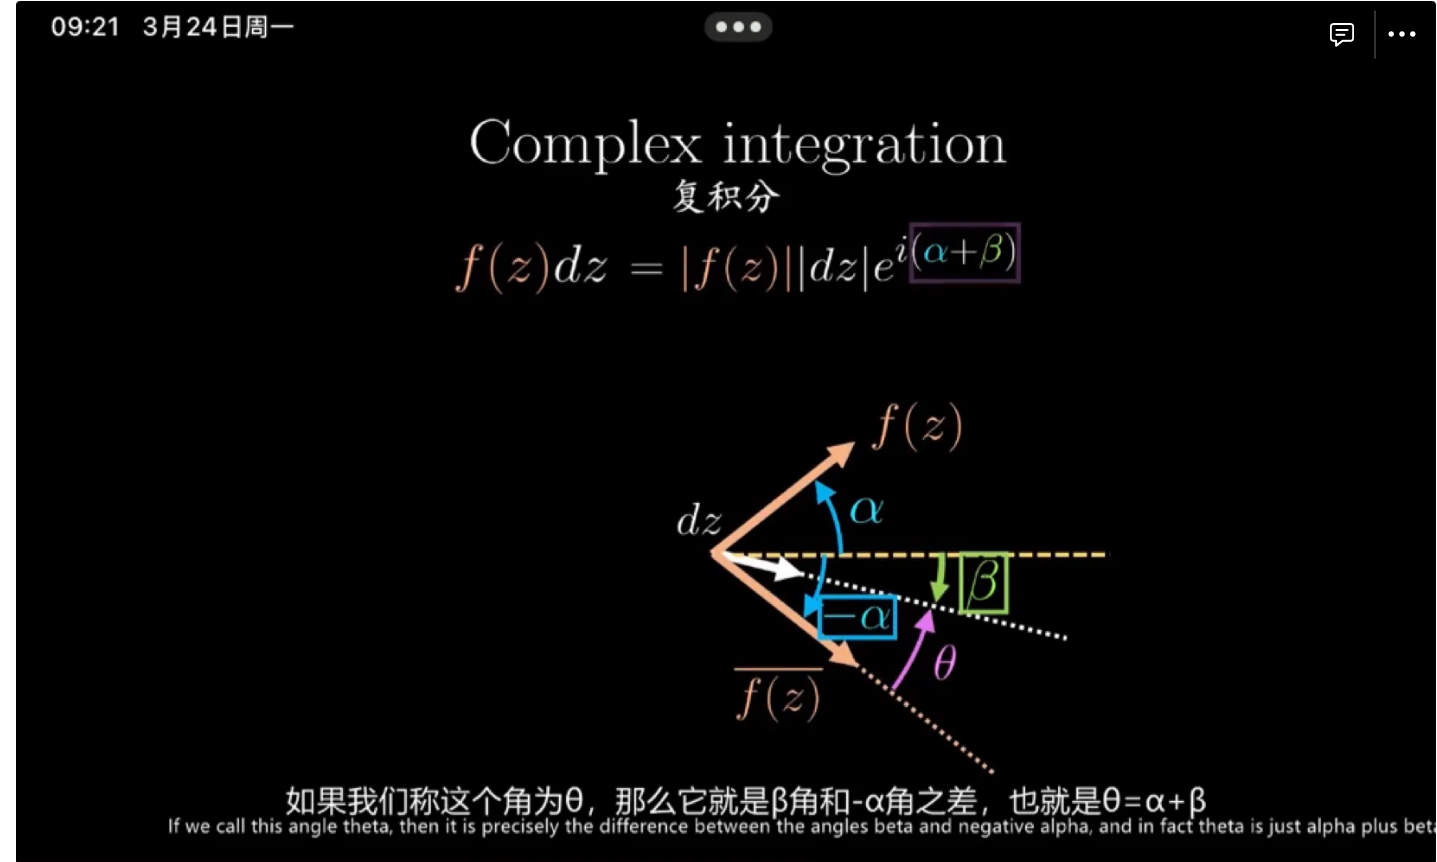
\includegraphics[scale=0.3]{image/1.jpeg}
\end{center}
这里用的是复数乘法：模相乘，辐角相加。记 $f(z)$ 的辐角为 $\alpha$，
$dz$ 的辐角为 $\beta$，由于符号相反，它们相加正好得到 $\theta$。
从共轭角的角度可以看出有关系式
\[
\theta - \alpha = \beta.
\]
因此，引入的核心思想就是：把 $f(z)$ 与 $dz$ 辐角的和，转化为
$\overline{f(z)}$ 与 $dz$ 的夹角 $\theta$。这样我们便可以写成
\[
e^{i\theta} = \cos\theta + i \sin\theta.
\]

当看到两个数的模相乘，再乘上它们夹角的余弦值时，自然会联想到点乘：
这正如力与位移的点积，表示在同一方向上的投影。
\begin{center}
    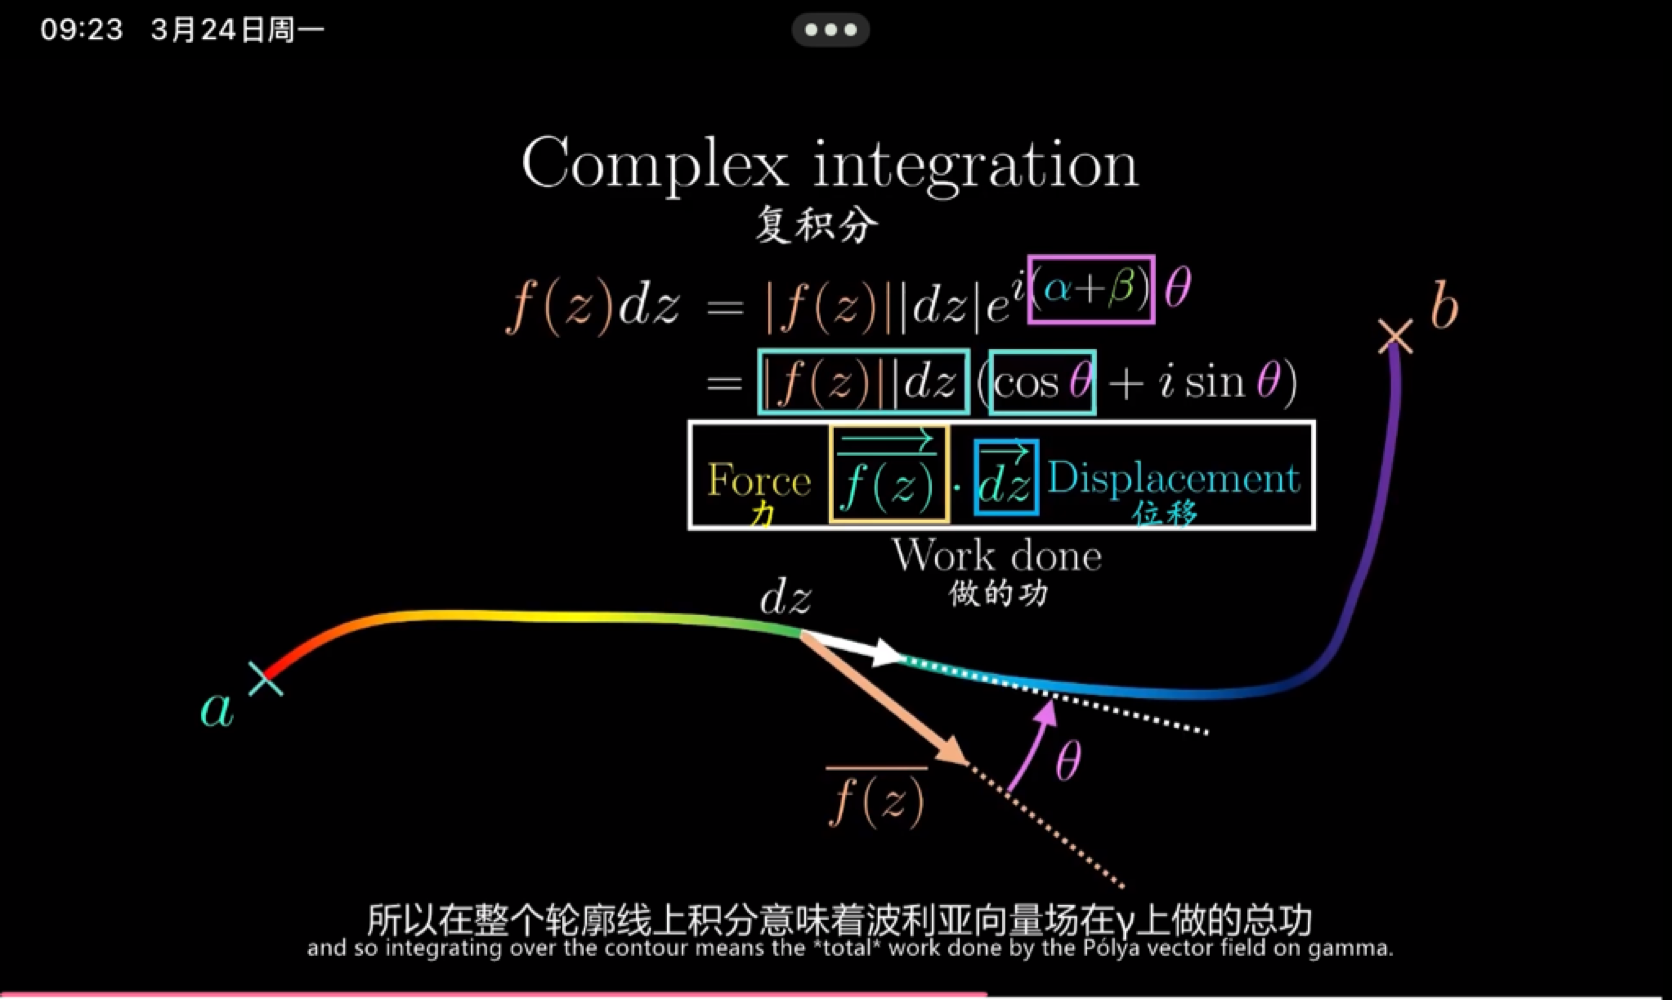
\includegraphics[width=0.75\paperwidth]{figure/workdone.png}
\end{center}
\begin{definition}[Pólya   波利亚向量场]
设复函数 $f(z)=u(x,y)+iv(x,y)$，$z=x+iy$。定义
\[
\mathbf P_f(x,y):=\begin{pmatrix}u(x,y)\\ -\,v(x,y)\end{pmatrix}.
\]
波利亚向量场，对于每一个点z我们取f(z)共轭作为附在z上的向量。要知道我们构造这个向量场就是或者说发明共轭就是吧辐角相加问题转化为两个向量夹角的问题。
\end{definition}
\begin{center}
    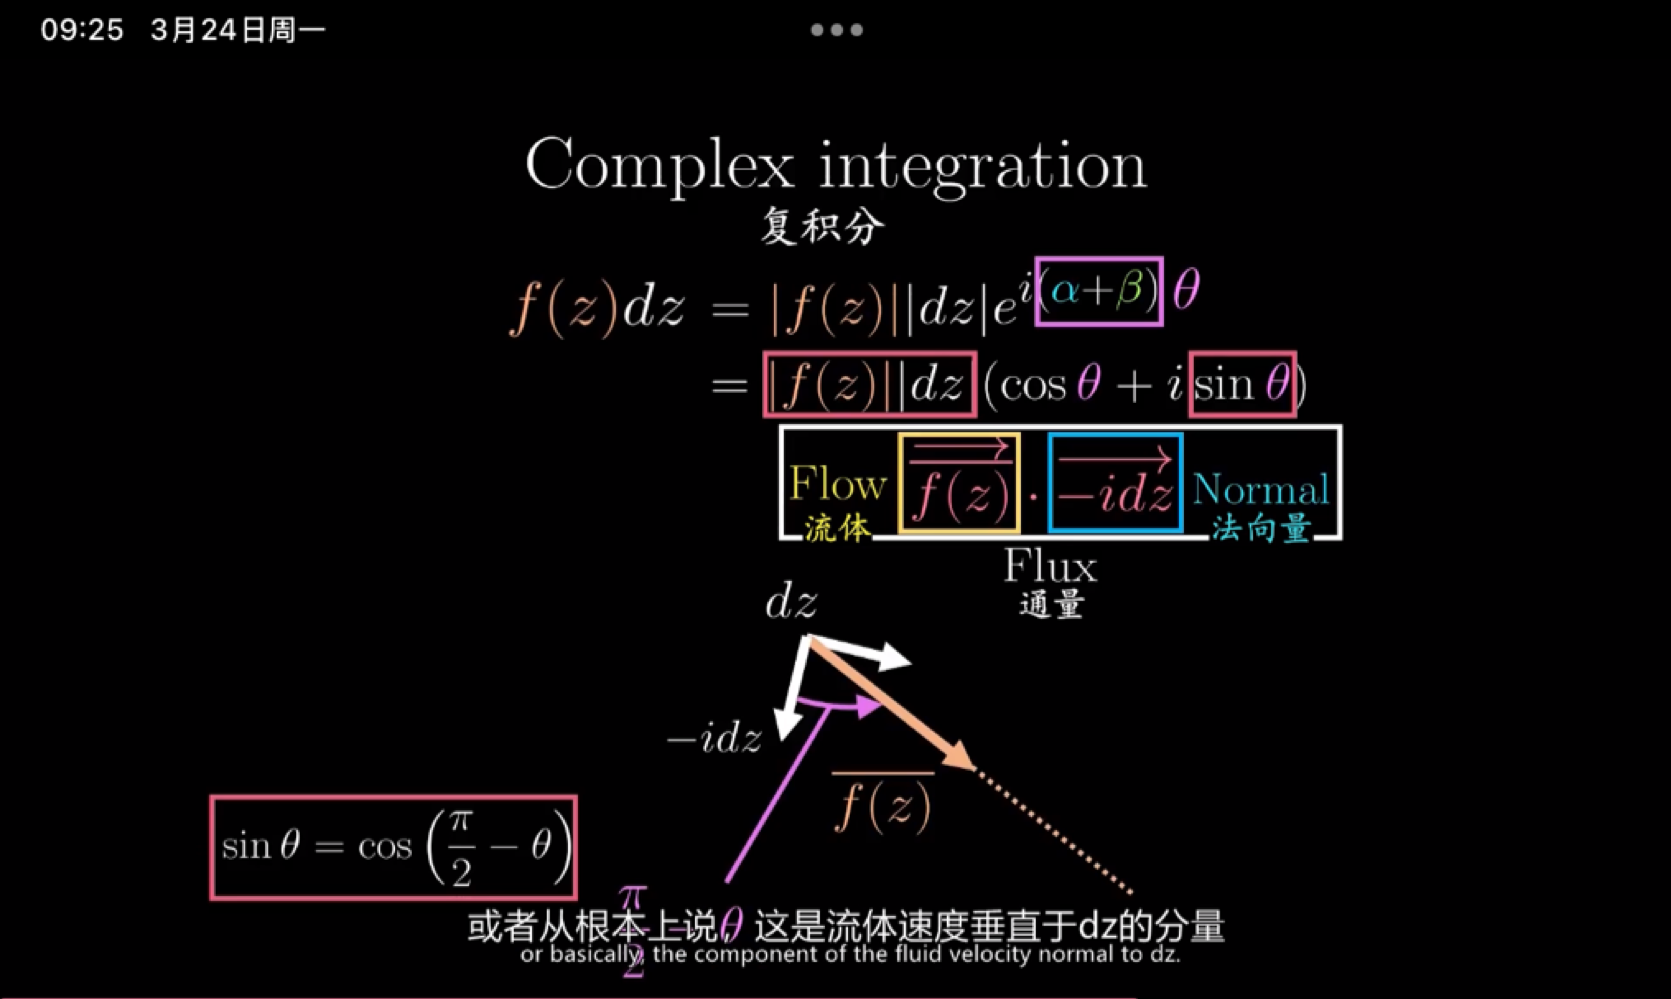
\includegraphics[width=0.75\paperwidth]{image/IMG_3358.PNG}
\end{center}
\begin{dxtips}
    在图中选择的是法向量 $-i\,dz$，它对应将切向量 $dz$ 顺时针旋转 $90^\circ$，即指向“向下/向外”的方向，
因此公式中自然写成 $-i\,dz$。在分解时，$\cos\theta$ 表示沿切向方向的投影分量，
而 $\sin\theta$ 表示沿法向方向的投影分量。
\end{dxtips}
\begin{proposition}
设 $f(z)$ 在曲线 $\gamma$ 上连续，则 $\displaystyle \int_\gamma f(z)\,dz$ 满足以下性质：
\begin{enumerate}[(i)]
  \item 线性性：若 $\alpha,\beta \in \mathbb{C}$，则
  \[
    \int_\gamma \bigl( \alpha f(z) + \beta g(z) \bigr)\,dz
    = \alpha \int_\gamma f(z)\,dz + \beta \int_\gamma g(z)\,dz.
  \]

  \item 反向性：如果 $\gamma^{-}$ 表示 $\gamma$ 的负向曲线，则
  \[
    \int_{\gamma^-} f(z)\,dz = -\int_\gamma f(z)\,dz.
  \]

  \item 长度估计：有不等式
  \[
    \left|\int_\gamma f(z)\,dz\right|
    \le \sup_{z\in\gamma} |f(z)| \cdot \operatorname{length}(\gamma).
  \]
\end{enumerate}
\end{proposition}
\section{柯西定理前的准备知识}
\begin{theorem}复平面上的不定积分]
若连续函数 $f$ 在区域 $\Omega$ 上具有原函数 $F$，$\gamma$ 是 $\Omega$ 内分别以 $w_1$ 和 $w_2$ 为起止点的曲线，那么
\[
\int_{\gamma} f(z)\,dz = F(w_2) - F(w_1).
\]
\end{theorem}
\begin{proof}
如果 $\gamma$ 是光滑的，此证明仅仅是链式法则和微积分的基本定理的简单应用。事实上，如果 
\[
z(t):[a,b]\to \mathbb{C}
\]
是曲线 $\gamma$ 的参数化法，那么 $z(a)=w_1,\;z(b)=w_2$，则
\[
\int_{\gamma} f(z)\,dz 
= \int_a^b f(z(t))\,z'(t)\,dt
= \int_a^b F'(z(t))\,z'(t)\,dt
= \int_a^b \frac{d}{dt}F(z(t))\,dt
= F(z(b))-F(z(a)).
\]

如果 $\gamma$ 只是分段光滑的，那么跟前面的讨论类似，可以得到一个可加和
\[
\int_{\gamma} f(z)\,dz 
= \sum_{k=0}^{n-1} \Big(F(z(a_{k+1}))-F(z(a_k))\Big)
= F(z(a_n))-F(z(a_0))
= F(z(b))-F(z(a)).
\]
\end{proof}
\begin{corollary}[闭合曲线积分为零的情况]
如果 $\gamma$ 是开集 $\Omega$ 上的封闭曲线，函数 $f$ 连续且在 $\Omega$ 上存在原函数，那么
\[
\int_{\gamma} f(z)\,dz = 0.
\]

这是因为封闭曲线的起止点重合了。
\end{corollary}
\begin{corollary}全纯函数导数是0就是常函数]
如果在区域 $\Omega$ 上 $f$ 是全纯函数，且 $f' = 0$，那么 $f$ 是常数。
\end{corollary}

\begin{proof}
取定一点 $w_0 \in \Omega$。只要证明对任一点 $w \in \Omega$ 都有 
\[
f(w) = f(w_0)
\]
即可。

因为 $\Omega$ 是连通的，所以对任意一点 $w \in \Omega$ 总存在分别以 $w_0$ 和 $w$ 为起止点的曲线 $\gamma$。又因为 $f$ 是全纯函数，$f$ 一定是函数 $f'$ 的原函数，因此
\[
\int_{\gamma} f'(z)\,dz = f(w) - f(w_0).
\]

根据假设 $f' = 0$，所以上述积分为零，即 $f(w) = f(w_0)$。
\end{proof}
\subsection{Goursat定理}
\begin{theorem}[定理 1.1]
如果 $\Omega$ 是复数集 $\mathbb{C}$ 中的开集，且 $T \subset \Omega$ 是三角形周线，其内部也包含在 $\Omega$ 中，那么
\[
\int_{T} f(z)\,dz = 0,
\]
其中 $f$ 在开集 $\Omega$ 上是全纯函数。
\end{theorem}
\begin{proof}
    

\begin{center}
    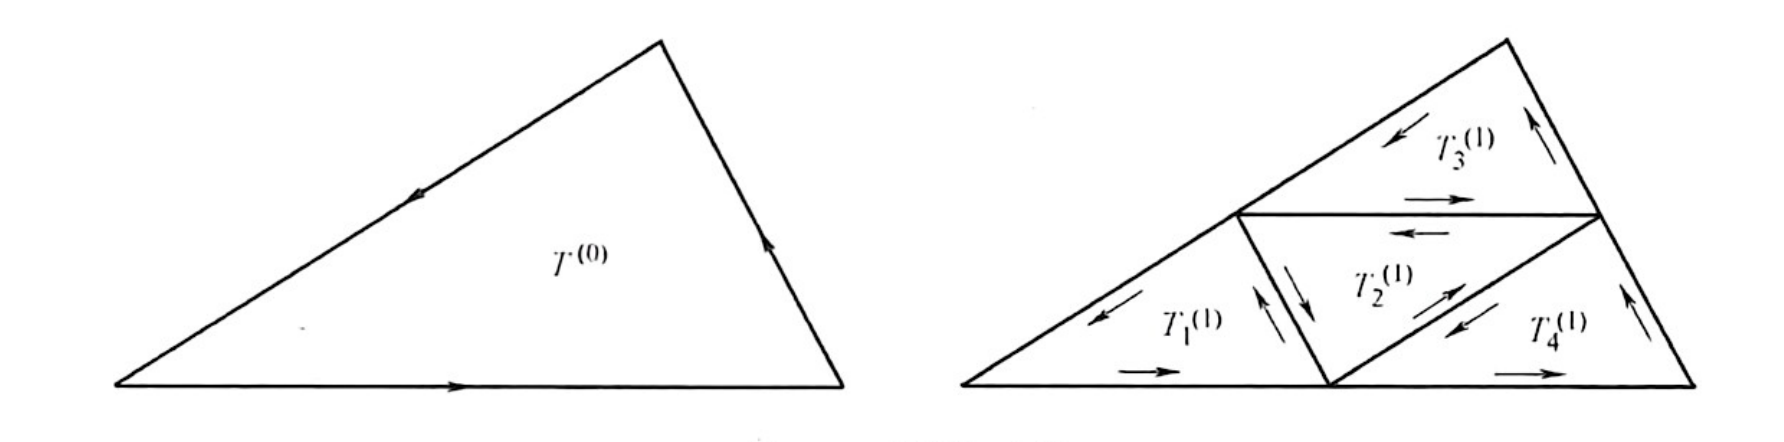
\includegraphics[width=0.75\paperwidth]{image/triangle.png}
\end{center}
第一步先把一个大三角形拆分成四个全等的小三角形。
因为每一条连接中点的线段积分时都从彼此正好相反的方向取了两次，刚好相互抵消，所以
\[
\int_{T^{(0)}} f(z)\,dz 
= \int_{T^{(1)}_1} f(z)\,dz 
+ \int_{T^{(1)}_2} f(z)\,dz 
+ \int_{T^{(1)}_3} f(z)\,dz 
+ \int_{T^{(1)}_4} f(z)\,dz. \tag{2}
\]

则至少存在某个 $j$ 满足
\[
\left| \int_{T^{(0)}} f(z)\,dz \right|
\leq 4 \left| \int_{T^{(1)}_j} f(z)\,dz \right|.
\]
假设大三角形的积分值是 $M$。由于大三角形的积分等于四个小三角形积分之和，所以必然存在一个小三角形的积分满足
\[
\left| \int_{\Delta^{(1)}} f(z)\,dz \right| \geq \frac{M}{4}.
\]
我们称这个性质为性质 $P$。因为如果四个积分都小于 $\tfrac{M}{4}$，那么它们的和一定小于 $M$，与假设矛盾。

此时我们把具有性质 $P$ 的小三角形拿出来，再将它分解为四个更小的全等三角形，再从中选出具有性质 $P$ 的三角形，如此不断分解下去。

于是，第 $n$ 轮具有性质 $P$ 的小三角形积分应满足

\[
\left| \int_{\Delta^{(n)}} f(z)\,dz \right| \geq \frac{M}{4^n} 
\qquad (n = 0,1,2,\dots)
\]
这个三角形会不断缩小缩小到一个点。这个是根据闭区间套定理的推广，嵌套紧集定理
\begin{theorem}[嵌套紧集定理（Cantor 型定理）]
设 $\{K_n\}$ 是一列非空紧集，满足
\[
K_1 \supseteq K_2 \supseteq K_3 \supseteq \cdots,
\]
并且直径满足
\[
\operatorname{diam}(K_n) \to 0 \quad (n \to \infty),
\]
则有
\[
\bigcap_{n=1}^\infty K_n = \{z_0\},
\]
其中 $z_0$ 是某个唯一的点。
\end{theorem}

存在 $z_0$ 属于所有的 $\Gamma^{(n)}$，且函数 $f$ 在 $z_0$ 点是全纯的，可写成
因为 $f$ 在 $z_0$ 点可微，所以有
\[
\lim_{z \to z_0} \frac{f(z)-f(z_0)}{z-z_0} = f'(z_0).
\]
这意味着：
\[
\forall \varepsilon > 0, \ \exists \delta > 0 \quad \text{使得当 } |z-z_0| < \delta \text{ 时，}
\quad \left| \frac{f(z)-f(z_0)}{z-z_0} - f'(z_0) \right| < \varepsilon.
\]
两边同乘｜z-z0｜，得
\[
\left| f(z) - f(z_0) - (z-z_0) f'(z_0) \right| < \varepsilon |z-z_0|.
\]
又因 $|z-z_0| < \tfrac{U}{2^n}$，所以
\[
\left| f(z) - f(z_0) - (z-z_0) f'(z_0) \right|
< \frac{U}{2^n}\varepsilon.
\]
因为 $|z-z_0|$ 就是最小三角形的直径，设 $U$ 是最大三角形的直径，则有
\[
2^n |z-z_0| = U.
\]
这里就限制了 $f(z)$。对两边积分，$f(z)$ 的积分小于它的最大值乘以三角形的周长，即
\[
\left| \int_{\Delta^{(n)}} f(z)\,dz \right|
\leq \varepsilon |z-z_0| \cdot \frac{C}{2^n}
\leq \varepsilon \cdot \frac{U}{2^n} \cdot \frac{C}{2^n}
= \varepsilon \cdot \frac{UC}{4^n}.
\]

然后两边同乘 $4^n$，因为最后右边还有 $\varepsilon$ 留下，所以证明大三角形的积分是 $0$。
\end{proof}
\begin{dxtips}
    我们进行了一系列放缩是为了先从大三角形转化为小三角形最后是一个点上简化问题，进行放缩就是保证两边乘了4的n次方还能有无穷小量ε留下。第一次对f(z)的放缩产生了一个$1/2^{n}$,然后积分的时候放缩成最大值周线长度又产生一$1/2^{n}$。
\end{dxtips}

\begin{corollary}[推论 1.2]
如果 $f$ 是开集 $\Omega$ 中的全纯函数，$\Omega$ 中包含矩形周线 $R$ 及其内部，那么
\[
\int_{R} f(z)\,dz = 0.
\]
\end{corollary}

此推论很显然，只要连接矩形的一条对角线得到两个全等的三角形即可。
\begin{theorem}[定理 2.1]
定义在开圆盘上的全纯函数在该圆盘内具有原函数。
\end{theorem}




















\section{柯西定理与柯西积分公式}


\begin{theorem}[定理 2.2 圆盘上的柯西定理]
如果函数 $f$ 在圆盘内是全纯函数，那么
\[
\int_{\gamma} f(z)\,dz = 0,
\]
其中 $\gamma$ 是圆盘内的任意闭曲线。
\end{theorem}
\begin{center}
    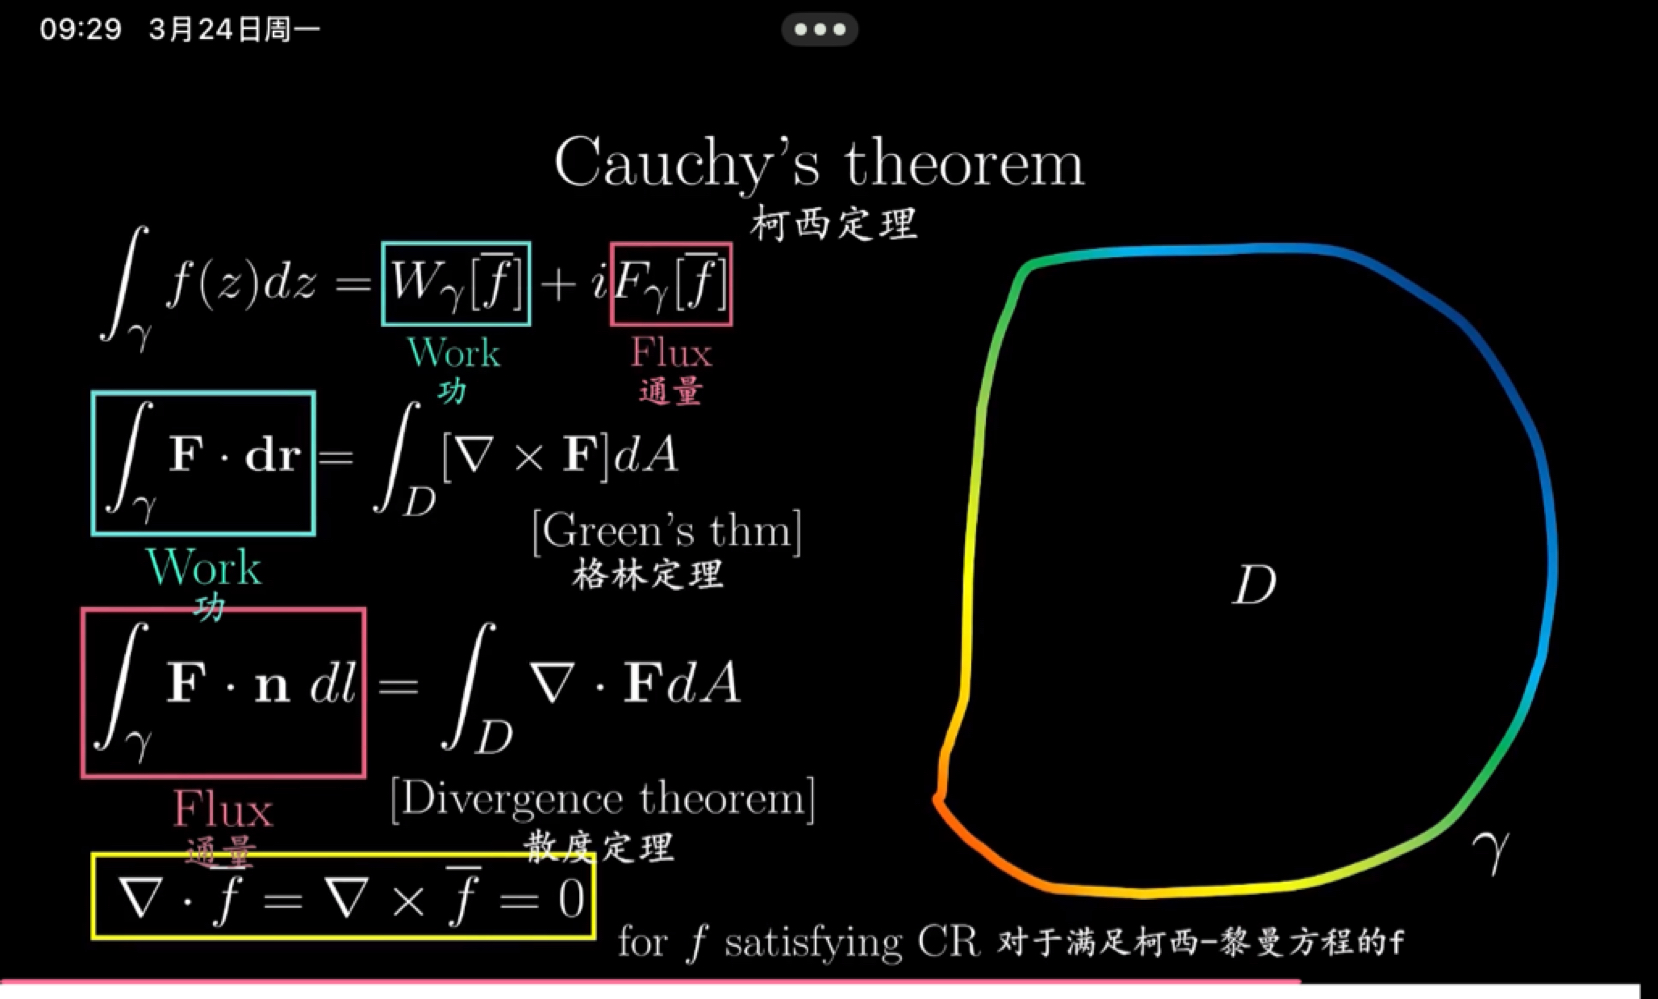
\includegraphics[width=0.75\paperwidth]{image/9.4.20.36.jpeg}
\end{center}
\begin{theorem}[定理 4.1 柯西积分公式]
假设函数 $f$ 在包含圆盘 $D$ 及其边界的开集中是全纯的，$C$ 表示圆盘的边界圆周，并且取正方向，那么对任意点 $z \in D$，有
\[
f(z) = \frac{1}{2\pi i} \int_{C} \frac{f(\zeta)}{\zeta - z}\, d\zeta .
\]
\end{theorem}
\begin{dxtips}
    柯西积分使得一个点上的函数值可以转化为一个线上的积分。f是全纯的，$f/{\zeta - z}$在就不是全纯的了，通过构造一个不是全纯的函数，来获取留数留数是什么后面自然会揭晓。
\end{dxtips}

\begin{corollary}[推论 4.2柯西积分公式高阶形式]
如果 $f$ 在开集 $\Omega$ 内是全纯的，那么 $f$ 在 $\Omega$ 内一定有无穷阶导数。
而且，如果 $C \subset \Omega$ 是一个圆周，其内部也在 $\Omega$ 内，那么
\[
f^{(n)}(z) = \frac{n!}{2\pi i} \int_{C} \frac{f(\zeta)}{(\zeta - z)^{\,n+1}} \, d\zeta,
\]
其中 $z$ 可以是 $C$ 内部的任意点。和前面定理中提到的一样，这里的圆周 $C$ 仍然取正向。
\end{corollary}

\begin{corollary}[推论 4.3 柯西不等式]
如果函数 $f$ 在包含圆盘 $D$ 的闭包的开集内是全纯的，圆盘 $D$ 的中心为 $z_0$，半径为 $R$，那么
\[
\bigl| f^{(n)}(z_0) \bigr| \leq \frac{n! \, \|f\|_{C}}{R^n},
\]
其中
\[
\|f\|_{C} = \sup_{z \in C} |f(z)|
\]
表示 $|f|$ 在圆周 $C$ 上的上确界。
\end{corollary}
\begin{theorem}[定理 4.4 幂级数的系数]
假设 $f$ 是定义在开集 $\Omega$ 内的全纯函数。如果 $D$ 是以 $z_0$ 为中心的圆盘，其闭包包含在 $\Omega$ 内，那么 $f$ 在 $z_0$ 点处展开成幂级数
\[
f(z) = \sum_{n=0}^{+\infty} a_n (z-z_0)^n,
\]
其中 $z \in D$，并且只要 $n \geq 0$，其系数为
\[
a_n = \frac{f^{(n)}(z_0)}{n!}.
\]
\end{theorem}
\begin{corollary}[推论 4.5 Liouville 定理]
如果 $f$ 是整函数并且有界，那么 $f$ 是常数。
\end{corollary}

\begin{proof}
因为复数集 $\mathbb{C}$ 是连通的，可以应用第 1 章中的推论 3.4，只要能证明 $f' = 0$ 即可。

对任意 $z_0 \in \mathbb{C}$，任意整数 $R > 0$，根据柯西不等式，有
\[
|f'(z_0)| \leq \frac{B}{R},
\]
其中 $B$ 是函数 $f$ 的界。只要令 $R \to +\infty$ 就可以证明 $f' = 0$。

这就完成了证明。事实上，代数学的基本定理可以很容易地由此推证。
\end{proof}
整函数在复平面是全纯的，保证了R可以取无限大。有界保证了B不能无限大。
\begin{corollary}[推论 4.6复系数多项式总有一个根]
任意一个非常数的具有复系数的多项式
\[
P(z) = a_n z^n + \cdots + a_0
\]
在复数集 $\mathbb{C}$ 内至少有一个根。
\end{corollary}
\begin{proof}
用反证法，假设 $P$ 没有根，那么 $1/P(z)$ 是有界的全纯函数。不妨假设 $a_n \neq 0$，多项式函数变形为
\[
\frac{P(z)}{z^n} = a_n + \left( \frac{a_{n-1}}{z} + \cdots + \frac{a_0}{z^n} \right),
\]
只要 $z \neq 0$。因为当 $|z|\to +\infty$ 时括号内的每一项都趋于 $0$，可以推出存在 $R>0$，令 $c = |a_n|/2$，只要 $|z| > R$，那么
\[
|P(z)| \geq c |z|^n.
\]

特别地，当 $|z| > R$ 时，$P$ 的倒数是有界的。又因为 $P$ 是连续的，在圆盘 $|z|\leq R$ 内没有根，所以在 $|z|\leq R$ 内 $P$ 的倒数也是有界的。因此函数 $1/P(z)$ 在整个复数集上都是有界的。

根据 Liouville 定理，$1/P$ 是常数，这与题设 $P$ 不是常数矛盾，所以原假设不成立。
\end{proof}

\begin{corollary}[推论 4.7因式分解定理]
任意一个阶数为 $n \geq 1$ 的多项式函数
\[
P(z) = a_n z^n + \cdots + a_0
\]
在复数集 $\mathbb{C}$ 上有 $n$ 个根。如果它的 $n$ 个根分别记为 $w_1, \cdots, w_n$，那么多项式函数 $P$ 就可以写成
\[
P(z) = a_n (z-w_1)(z-w_2)\cdots(z-w_n).
\]
\end{corollary}
\begin{dxtips}
    推论4.6 4.7都是为留数做准备
\end{dxtips}
\begin{theorem}[定理 4.8 恒等定理]
假设 $f$ 是区域 $\Omega$ 上的全纯函数，如果存在 $\Omega$ 内的某个数列，
且其极限点也在 $\Omega$ 内，使得 $f$ 在该数列上的值都为 $0$，
那么函数 $f$ 就等于 $0$。

也就是说，如果全纯函数 $f$ 在连通的开集 $\Omega$ 内的零点在 $\Omega$ 内累积，那么 $f \equiv 0$。
\end{theorem}
0会扩散。
\begin{corollary}[推论 4.9]
假设 $f$ 和 $g$ 都是区域 $\Omega$ 上的全纯函数，在 $\Omega$ 的某个非空开子集中
（或者更一般的，以 $\Omega$ 内的点为极限点的数列上）恒有 $f(z)=g(z)$，
那么，在整个 $\Omega$ 上恒有 $f(z)=g(z)$。

假设给出两个函数 $f$ 和 $F$，它们分别在区域 $\Omega$ 和 $\Omega'$ 上解析，
且 $\Omega \subset \Omega'$。如果这两个函数在 $\Omega$ 上是一致的，那么称
$F$ 是函数 $f$ 在集合 $\Omega'$ 上的解析延拓。上面的推论保证了解析延拓的唯一性，
因此函数 $F$ 是由 $f$ 唯一确定的。
\end{corollary}


下面的定理是柯西定理的逆定理。

\begin{theorem}[Morera 定理定理 5.1]
假设 $f$ 在开圆盘 $D$ 上是连续函数，如果对包含在 $D$ 内的任意三角形周线 $T$ 均有
\[
\int_{T} f(z)\,dz = 0,
\]
那么函数 $f$ 是全纯的。
\end{theorem}

\begin{proof}
根据定理 2.1 的证明，函数 $f$ 在 $D$ 上有原函数 $F$ 满足 $F' = f$。  
根据正则性定理，函数 $F$ 是可复微的，所以 $f$ 是全纯的。
\end{proof}
\begin{theorem}[5.2全纯性质可以通过一致收敛传递]
如果 $\{ f_n \}_{n=1}^{+\infty}$ 是一列全纯函数，在 $\Omega$ 中的每一个紧子集上都一致收敛于函数 $f$，那么函数 $f$ 是全纯的。
\end{theorem}
\begin{theorem}[5.3]
在定理 5.2 的条件下，导函数列 $\{ f_n' \}_{n=1}^{+\infty}$ 在 $\Omega$ 中的每一个紧子集上都一致收敛于函数 $f'$。
\end{theorem}
\chapter{幂级数}
\section{幂级数基本知识}stein  的第二章书本的第四章
\begin{proposition}
在圆域 $|z| < 1$ 内，几何级数
\[
\sum_{n=0}^{+\infty} z^n
\]
是绝对收敛的，并且其和函数为
\[
\frac{1}{1-z},
\]
此函数在开集 $\mathbb{C} \setminus \{1\}$ 上是全纯的。

证明：首先计算其部分和
\[
\sum_{n=0}^{N} z^n = \frac{1 - z^{N+1}}{1-z}.
\]
当 $|z| < 1$ 时，显然有
\[
\lim_{N \to +\infty} z^{N+1} = 0,
\]
于是得出结论。
\end{proposition}
\begin{definition}
幂级数可写成下列形式
\[
\sum_{n=0}^{+\infty} a_n z^n,
\]
其中 $a_n \in \mathbb{C}$。要考察此级数是否绝对收敛，就是要研究级数
\[
\sum_{n=0}^{+\infty} \lvert a_n \rvert \, \lvert z^n \rvert
\]
是否收敛。
\end{definition}
\begin{theorem}[2.5收敛半径内绝对收敛]
对任意的幂级数，必存在 $0 \leq R \leq +\infty$ 使得  
\begin{enumerate}[(i)]
  \item 如果 $|z| < R$，级数绝对收敛；
  \item 如果 $|z| > R$，级数发散。
\end{enumerate}
如果规定 $1/0 = +\infty, \; 1 / +\infty = 0$，那么 $R$ 由 Hadamard 公式给出，即
\[
\frac{1}{R} = \limsup_{n \to \infty} \lvert a_n \rvert^{1/n}.
\]

其中，数 $R$ 称为幂级数的\textbf{收敛半径}，区域 $|z| < R$ 称为\textbf{收敛圆盘}。特别地，指数函数的幂级数的收敛半径 $R = +\infty$，几何级数的收敛半径 $R = 1$。
\end{theorem}
\begin{theorem}[2.6函数和自己的导数的收敛半径一样大]
幂级数
\[
f(z) = \sum_{n=0}^{+\infty} a_n z^n
\]
是定义在其收敛圆盘上的全纯函数。它的导数依然是一个幂级数，是由函数 $f$ 的幂级数逐项求导得到的，即
\[
f'(z) = \sum_{n=0}^{+\infty} n a_n z^{n-1}.
\]
所以，$f'$ 与 $f$ 具有相同的收敛半径。
\end{theorem}
\section{收敛判定}
\begin{theorem}[Weierstrass 判别法]
设 $f_n(z)\,(n=1,2,3,\dots)$ 在复平面点集 $E$ 上有定义，并且设
\[
a_1 + a_2 + \cdots + a_n + \cdots
\]
是收敛的正项级数。若在 $E$ 上
\[
|f_n(z)| \leq a_n \quad (n=1,2,3,\dots),
\]
那么级数 $(2.1)$ 在 $E$ 上一致收敛。
\end{theorem}
用一个收敛的数列限制函数列。
\begin{theorem}[Cauchy--Hadamard 定理柯西阿玛达]
设幂级数
\[
\sum_{n=0}^{\infty} a_n x^n,
\]
令
\[
R = \frac{1}{\limsup\limits_{n \to \infty} \sqrt[n]{|a_n|}}.
\]

则有：
\begin{enumerate}
  \item 当 $R = 0$ 时，级数在 $x=0$ 处绝对收敛，在 $\mathbb{R} \setminus \{0\}$ 上发散；
  \item 当 $R = +\infty$ 时，级数在 $\mathbb{R}$ 上绝对收敛；
  \item 当 $R \in \mathbb{R}^+$ 时，级数在 $(-R,R)$ 上绝对收敛，在 $(-\infty,-R) \cup (R,+\infty)$ 上发散。
\end{enumerate}
\end{theorem}
\begin{proof}[证明（柯西根值判别法）]
当 $x=0$ 时显然绝对收敛。设 $x \neq 0$。根据 Abel 第一准则，只需讨论
\[
\sum_{n=0}^{\infty} |a_n x^n|
\]
的收敛性。令
\[
q = \limsup_{n \to \infty} \sqrt[n]{|a_n x^n|}
   = |x| \cdot \limsup_{n \to \infty} \sqrt[n]{|a_n|}.
\]

由定义有
\[
\frac{1}{R} = \limsup_{n \to \infty} \sqrt[n]{|a_n|}.
\]

因此：
\begin{enumerate}
  \item 若 $R = 0$，则 $q = +\infty$，除 $x=0$ 外级数在 $\mathbb{R}$ 上发散；
  \item 若 $R = +\infty$，则 $q = 0$，级数在 $\mathbb{R}$ 上绝对收敛；
  \item 若 $R \in \mathbb{R}^+$，则
  \[
  q = |x| \cdot \frac{1}{R} = \frac{|x|}{R}.
  \]
  若 $|x| < R$，则 $q < 1$，此时级数绝对收敛；若 $|x| > R$，则 $q > 1$，此时级数发散。
\end{enumerate}

综上，定理得证。
\end{proof}
\begin{dxtips}
    R的式子就是为了把R放在分母上
\end{dxtips}
\begin{theorem}[柯西根值判别法]
设正项级数 $\sum_{n=1}^{\infty} a_n$。
\begin{enumerate}
  \item 当 $n$ 充分大时，若 $\sqrt[n]{a_n} \leq q$，其中 $0 < q < 1$，则级数收敛；
  \item 若存在无穷多个 $n$ 满足 $\sqrt[n]{a_n} \geq 1$，则级数发散。
\end{enumerate}
\end{theorem}

\begin{proof}
(1) 若 $0 < q < 1$，则几何级数 $q^n$ 收敛。当 $n$ 充分大时，由条件可知
\[
\sqrt[n]{a_n} \leq q \quad \Longrightarrow \quad a_n \leq q^n.
\]
由正项级数的比较判别法可知 $\sum_{n=1}^{\infty} a_n$ 收敛。

(2) 若存在无穷多个 $n$ 满足 $\sqrt[n]{a_n} \geq 1$，则 $a_n \not\to 0$，于是可知 $\sum_{n=1}^{\infty} a_n$ 发散。
\end{proof}

\begin{theorem}[柯西根值判别法的极限形式]
设正项级数 $\sum_{n=1}^{\infty} a_n$，令
\[
\limsup_{n \to \infty} \sqrt[n]{a_n} = q.
\]
则有：
\begin{enumerate}
  \item 当 $q < 1$ 时，级数收敛；
  \item 当 $q > 1$ 时，级数发散。
\end{enumerate}
\end{theorem}
根值判别法也就是与几何级数的比较比如1/2的n次方级数。极限形式就是最大的开n次根
\begin{theorem}[达朗贝尔判别法]
设 $\sum_{n=0}^{\infty} c_n$ 是一个正项级数，若极限
\[
\lambda = \lim_{n \to \infty} \left| \frac{c_{n+1}}{c_n} \right|
\]
存在，则：
\begin{enumerate}
  \item 若 $\lambda < 1$，则级数收敛；
  \item 若 $\lambda > 1$，则级数发散；
  \item 若 $\lambda = 1$，则判别无效。
\end{enumerate}
\end{theorem}

\chapter{留数}
\begin{definition}[留数]
设函数 $f(z)$ 在点 $z_0$ 的去心邻域 $0<|z-z_0|<r$ 内解析，则 $f(z)$ 可展开为
\[
f(z) = \sum_{n=-\infty}^{\infty} a_n (z-z_0)^n,
\]
其中 $a_n$ 是洛朗级数系数。特别地，系数
\[
\operatorname{Res}(f, z_0) := a_{-1}
\]
称为函数 $f$ 在点 $z_0$ 的\textbf{留数}。
\end{definition}

在复分析中，residue 是函数在某个孤立奇点附近积分环绕时“留下的值” —— 一种“局部残余信息”，所以residue = 留下的量，这个词根含义恰好与其数学意义吻合。\textbf{将复杂的路径积分问题转化为奇点处留数的代数计算}。
那我们首先要弄清楚有什么样的奇点。
\section{零点与奇点}
\begin{definition}[孤立奇点Isolated singularity]
    根据定义，函数 $f$ 的奇点是指，复数 $z_0$ 使得函数在 $z_0$ 的去心邻域内有定义，
而在 $z_0$ 点处没有定义。也可以称这样的点为\textbf{孤立奇点}。例如，如果函数 $f$
在有孔平面上定义为
\[
f(z) = z
\]
那么原点就是它的奇点。
\end{definition}一句话来说去心领域有定义，z0处没有定义
\begin{definition}[孤立奇点——可去奇点Removable singularity]
 如果将刚才例子中f(z)=z,将f在零点的定义为f(0)=0因此函数被延拓成连续的还是整的也就是说奇点被消除了，这就是可去奇点   
\end{definition}好好定义完了以后函数久变成连续而且整的0️⃣就是可去奇点
\begin{definition}[孤立奇点——极点]
  在有孔平面上的函数 $g(z) = \tfrac{1}{z}$。很显然，在零点函数 $g$ 不能延拓成连续的，
更不能变成全纯的。事实上，当 $z$ 逼近于 $0$ 时，$g(z)$ 是趋于无穷大的，
此时称原点为\textbf{极点}。  
\end{definition}
\begin{definition}[孤立奇点——本性奇点]
    最后，定义在有孔平面上的函数
\[
h(z) = e^{1/z},
\]
此时可去奇点和极点就不能完全说明问题了。事实上，当 $z$ 从正实轴方向趋于 $0$ 时，
$h(z)$ 趋于无穷；当 $z$ 从负实轴方向趋于 $0$ 时，$h(z)$ 趋于 $0$；
当 $z$ 从虚轴上趋于 $0$ 时，$h(z)$ 强烈振动，但仍然是有界的。
这就是所谓的\textbf{本性奇点}。
\end{definition}
\begin{definition}[零元]
 因为奇点的产生通常源于分母趋于 $0$，所以我们就首先对全纯函数的零元进行局部研究。

如果全纯函数在点 $z_0$ 处满足 $f(z_0)=0$，称复数 $z_0$ 为全纯函数的\textbf{零元}。
特别地，研究表明，非平凡全纯函数的零点就是孤立的。换句话说，如果函数 $f$
在 $\Omega$ 上是全纯的，且对某点 $z_0 \in \Omega$ 满足 $f(z_0)=0$，那么存在
在 $z_0$ 的开邻域 $U$ 使得函数当 $z \in U \setminus \{z_0\}$ 时满足 $f(z)\neq 0$
（除非 $f$ 恒等于零）。

下面就开始对全纯函数在零元附近进行局部描述。   
\end{definition}
\begin{theorem}[1.1]
假设函数 $f$ 在连通的开集 $\Omega$ 上是全纯的，$z_0 \in \Omega$ 是它的零元，
并且 $f$ 在 $\Omega$ 上不恒等于 $0$。那么存在 $z_0$ 的邻域 $U \subset \Omega$ 
和定义在 $U$ 上的非零函数 $g$，同时存在唯一的正整数 $n$，使得对所有的 
$z \in U$，有
\[
f(z) = (z - z_0)^n g(z).
\]
\end{theorem}
\begin{theorem}[1.2]
如果 $z_0 \in \Omega$ 是 $f$ 的极点，那么在 $z_0$ 的某邻域中存在非零的全纯函数 $h$ 
和唯一的正整数 $n$ 使得
\[
f(z) = (z - z_0)^{-n} h(z).
\]
\end{theorem}
\begin{theorem}[1.3]
如果 $z_0$ 点是函数 $f$ 的 $n$ 阶极点，那么
\[
f(z) = \frac{a_{-n}}{(z-z_0)^n}
      + \frac{a_{-n+1}}{(z-z_0)^{n-1}}
      + \cdots
      + \frac{a_{-1}}{(z-z_0)}
      + G(z),
\tag{1}
\]
其中，$G$ 是定义在 $z_0$ 的某邻域中的全纯函数。
\end{theorem}
\section{留数公式}
\begin{theorem}[2.1]
假设函数 $f$ 在包含圆周 $C$ 及其内部的开集中，除了极点 $z_0$ 外，是全纯的。那么
\[
\int_{C} f(z)\,dz = 2\pi i \,\operatorname{Res}_{z_0} f.
\]
\end{theorem}
\begin{proof}
这里也要用到锁眼周线来消除极点，令走廊的宽度趋于零，那么
\[
\int_{C} f(z)\,dz = \int_{C_\varepsilon} f(z)\,dz,
\]
其中，$C_\varepsilon$ 是以 $z_0$ 为中心，$\varepsilon$ 为半径的小圆周。

注意到，根据柯西积分公式（上一章的定理 4.1）将其应用到常函数 $f = a_{-1}$ 上，很容易推出
\[
\frac{1}{2\pi i} \int_{C_\varepsilon} \frac{a_{-1}}{z-z_0}\,dz = a_{-1}.
\]

类似地，当 $k > 1$ 时，应用相应的求导公式（上一章的推论 4.2）得
\[
\frac{1}{2\pi i} \int_{C_\varepsilon} \frac{a_{-k}}{(z-z_0)^k}\,dz = 0.
\]

但是，在 $z_0$ 的邻域中
\[
f(z) = \frac{a_{-n}}{(z-z_0)^n}
     + \frac{a_{-n+1}}{(z-z_0)^{n-1}}
     + \cdots
     + \frac{a_{-1}}{z-z_0}
     + G(z),
\]
其中，$G$ 是全纯的。根据柯西定理，
\[
\int_{C_\varepsilon} G(z)\,dz = 0,
\]
因此
\[
\int_{C_\varepsilon} f(z)\,dz = 2\pi i\, a_{-1}.
\]
定理得证。
\end{proof}
\begin{proposition}[一阶极点的留数公式]
设 $z_0$ 是函数 $f(z)$ 的一个一阶极点。

(1) 若 $f(z)$ 可写为
\[
f(z) = \frac{1}{z-z_0}\,\varphi(z),
\]
其中 $\varphi(z)$ 在 $z_0$ 附近解析，且 $\varphi(z_0) \neq 0$，则
\[
\operatorname{Res}(f,z_0) = \lim_{z \to z_0} (z-z_0)f(z) = \varphi(z_0).
\]

(2) 若 $f(z)$ 可写为有理型
\[
f(z) = \frac{P(z)}{Q(z)},
\]
其中 $P(z)$ 与 $Q(z)$ 在 $z_0$ 附近解析，且 $P(z_0) \neq 0$，并且 $z_0$ 是 $Q(z)$ 的一阶零点，则 $z_0$ 是 $f(z)$ 的一阶极点，且
\[
\operatorname{Res}(f,z_0) = \frac{P(z_0)}{Q'(z_0)}.
\]
\end{proposition}
这个对f(z)长的样子是有特殊要求的，上面的z0处≠0而且解析，下面处了z0是一级0点没有其他0点，留数就是P(z0)/Q(z0)的导数
\begin{dxtips}
  因为把f(z)洛朗展开除了有1/(z-z0)的项全部都是全纯的积分都是零。就这项被留了下来。这一项的系数就是留数，其他部分积分就是2πi这里应该用参数法积。  
\end{dxtips}
\begin{proof}
由于 $z_0$ 是 $f(z)$ 的 $m$ 阶极点，所以在 $z_0$ 的某个去心邻域内的 Laurent 级数展开式为
\[
f(z) = c_{-m}(z-z_0)^{-m} + \cdots + c_{-2}(z-z_0)^{-2} + c_{-1}(z-z_0)^{-1} + c_0 + c_1(z-z_0) + \cdots.
\]

因此
\[
(z-z_0)^n f(z) = c_{-m}(z-z_0)^{n-m} + c_{-m+1}(z-z_0)^{n-m+1} + \cdots + c_{-1}(z-z_0)^{n-1} + \cdots.
\]

对上式求 $n-1$ 阶导数，得
\[
\frac{d^{\,n-1}}{dz^{\,n-1}} \big[ (z-z_0)^n f(z) \big]
= (n-1)! \, c_{-1} + (\text{含有 } z-z_0 \text{ 正幂的项}).
\]

所以
\[
\lim_{z \to z_0} \frac{d^{\,n-1}}{dz^{\,n-1}} \big[ (z-z_0)^n f(z) \big] = (n-1)! \, c_{-1}.
\]

于是
\[
\operatorname{Res}(f,z_0) = c_{-1} 
= \frac{1}{(n-1)!} \lim_{z \to z_0} \frac{d^{\,n-1}}{dz^{\,n-1}} \big[ (z-z_0)^n f(z) \big].
\]
\end{proof}
\begin{dxtips}
    因为要保证z=z0的时候 左边就只剩下留数不是0所以两边先乘 z的m阶导 此时留数的后面跟着z-z0的m减1要去掉z-z0来保证留数能留下所以要导m-1次
\end{dxtips}


从作业把精华拿出来

















\end{document}
